\documentclass[a4paper,12pt]{article}
\usepackage[russian]{babel}
\usepackage[utf8]{inputenc}
\usepackage{amsmath}
\usepackage{graphicx}
\usepackage{array}
\usepackage{makecell}
\usepackage{geometry}
\usepackage{float}
\usepackage{listings}
\usepackage{xcolor}
\usepackage{tocloft}
\usepackage{hyperref}

\geometry{left=2.5cm, right=2.5cm, top=2.5cm, bottom=2.5cm}

\definecolor{codegray}{gray}{0.9}
\lstset{
    backgroundcolor=\color{codegray},
    basicstyle=\ttfamily\small,
    frame=single,
    breaklines=true
}

\renewcommand{\cftsecleader}{\cftdotfill{\cftdotsep}}
\renewcommand{\contentsname}{Оглавление}

\begin{document}

\begin{titlepage}
    \centering
    \vspace*{1cm}
    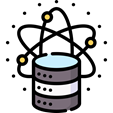
\includegraphics[width=0.25\textwidth]{media/image1.png}\hfill
    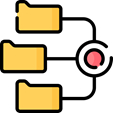
\includegraphics[width=0.25\textwidth]{media/image2.png}\hfill
    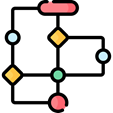
\includegraphics[width=0.25\textwidth]{media/image3.png}
    
    \vspace{3cm}
    
    {\fontsize{54}{28}\bfseries Структуры данных\par}
    \vspace{0.7cm}
    {\fontsize{54}{28}\bfseries и алгоритмы\par}
    
    \vspace{3cm}
    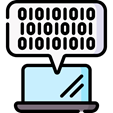
\includegraphics[width=0.25\textwidth]{media/image4.png}\hfill
    
\includegraphics[width=0.25\textwidth]{media/image5.png}\hfill
    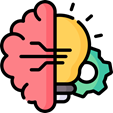
\includegraphics[width=0.25\textwidth]{media/image6.png}
    
    \vfill
\end{titlepage}

\tableofcontents
\newpage

\section{Оценки алгоритмов}
\label{sec:оценки-алгоритмов}

Оценка алгоритмов --- это процесс анализа и сравнения алгоритмов для определения их эффективности в зависимости от размера входных данных $n$.

Для оценки алгоритмов используются разные нотации. Эти нотации нужны для оценки работы алгоритмов в худшем или лучшем случае или как себя введет алгоритм в среднем. Для этого нам нужно описать алгоритм $f(n)$ какой-то более простой функцией $g(n)$.

Виды нотаций:

\begin{itemize}
    \item \textbf{Верхняя граница} (худший случай или нотация О-большое): $f(n) = O(g(n))$, если существуют положительные константы $c$ и $n_{0}$ такие, что $0 \leq f(n) \leq c \cdot g(n)$ для всех $n \geq n_{0}$. Это означает, что алгоритм работает не медленнее, чем указанная функция.
    
    \item \textbf{Нижняя граница} (лучший случай или нотация Омега-большое): $f(n) = \Omega(g(n))$, если существуют положительные константы $c$ и $n_{0}$ такие, что $0 \leq c \cdot g(n) \leq f(n)$ для всех $n \geq n_{0}$. Это означает, что алгоритм работает не быстрее, чем указанная функция.
    
    \item \textbf{Точная граница} (средний случай или нотация Тета): $f(n) = \Theta(g(n))$, если существуют положительные константы $c_{1}$, $c_{2}$ и $n_{0}$ такие, что $0 \leq c_{1} \cdot g(n) \leq f(n) \leq c_{2} \cdot g(n)$ для всех $n \geq n_{0}$. Это означает, что алгоритм работает примерно так же, как указанная функция.
    
    \item \textbf{Строгая верхняя граница} (нотация о-малое): $f(n) = o(g(n))$, если для любой положительной константы $c > 0$ существует константа $n_{0} > 0$ такие, что $0 \leq f(n) < c \cdot g(n)$ для всех $n \geq n_{0}$. Это означает, что алгоритм работает существенно быстрее, чем указанная функция.
    
    \item \textbf{Строгая нижняя граница} (нотация омега-малое): $f(n) = \omega(g(n))$, если для любой положительной константы $c > 0$ существует константа $n_{0} > 0$ такие, что $0 \leq c \cdot g(n) < f(n)$ для всех $n \geq n_{0}$. Это означает, что алгоритм работает существенно быстрее, чем указанная функция.
\end{itemize}

Строгие оценки используются для более тонких асимптотических сравнений. Например, наш алгоритм можно описать функцией $f(n) = 2 \cdot n$ и мы пытаемся оценить его функцией $g(n) = n$. Тогда проверим следующие равенства:

\begin{itemize}
    \item $2 \cdot n = O(n)$ --- верно, так как мы можем подобрать константу $c$ такую, что будет выполняться неравенство.
    \item $2 \cdot n = o(n)$ --- неверно, так как неравенство должно выполняться для любой положительной константы $c$.
    \item $2 \cdot n = \Omega(n)$ --- верно, так как мы можем подобрать константу $c$ такую, что будет выполняться неравенство.
    \item $2 \cdot n = \omega(n)$ --- неверно, так как неравенство должно выполняться для любой положительной константы $c$.
\end{itemize}

Теперь рассмотрим какими функциями $g(n)$ мы можем оценивать алгоритм:

\begin{itemize}
    \item $g(n) = const$ --- константная сложность, алгоритм не зависит от размера входных данных и часто константу берут равной единице ($const = 1$).
    \item $g(n) = \log(n)$ --- логарифмическая сложность.
    \item $g(n) = n$ --- линейная сложность.
    \item $g(n) = n \cdot \log(n)$ --- линейно-логарифмическая сложность (квазилинейная сложность).
    \item $g(n) = n^{const}$ --- степенная сложность (полиномиальная сложность), частные случаи $n^{2}$ --- квадратичная сложность и $n^{3}$ --- кубическая сложность.
    \item $g(n) = {const}^{n}$ --- показательная сложность (экспоненциальная сложность) причем $c > 1$, частные случаи $2^{n}$ и $3^{n}$.
    \item $g(n) = n!$ --- факториальная сложность.
\end{itemize}

Вот график для сравнения функций оценок сложности:

\begin{figure}[H]
    \centering
    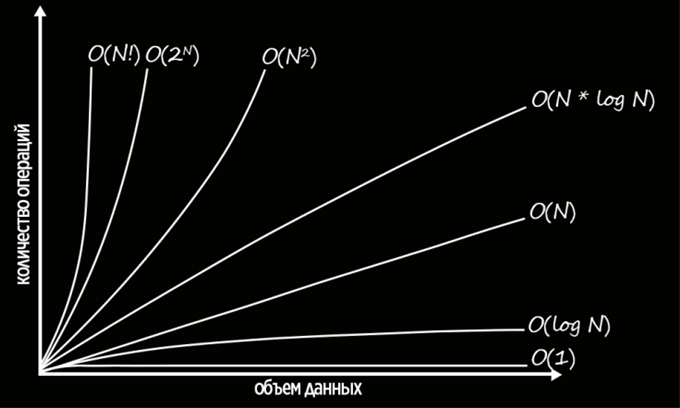
\includegraphics[width=0.9\textwidth]{media/image7.png}
    \caption{Сравнение функций оценок сложности}
\end{figure}

Такими оценками мы можем оценить скорость работы алгоритма (временная сложность алгоритма) или память необходимую алгоритму (пространственная сложность). Также подобные оценки используют не только для оценок алгоритмов, но во многих других сферах.

\subsection{Оценка скорости алгоритмов}
\label{subsec:оценка-скорости-алгоритмов}

Оценка скорости алгоритма или временная сложность, --- это мера того, как время выполнения алгоритма увеличивается с ростом размера входных данных $n$. С помощью этой оценки мы можем выбрать алгоритм, когда нам важна скорость работы.

\subsection{Оценка памяти необходимой алгоритмам}
\label{subsec:оценка-памяти-необходимой-алгоритмам}

Оценка памяти необходимой алгоритму или пространственная сложность --- это оценка объема памяти, которую алгоритм использует для своей работы в зависимости от размера входных данных $n$. Можем использовать данные оценки, если нам критически важно отслеживать память, используемую алгоритмом и наши ресурсы ограничены.

Также данные оценки могут показать использует ли алгоритм дополнительную память. Например, некоторые алгоритмы могут создавать копию входных данных и модернизировать именно эту копию и параллельно записывать правильно модернизированные данные во входные. Алгоритмы, которые работают без создания копий входных данных и меняют их непосредственно в оригинальном наборе, называют алгоритмами, работающими на месте.

\subsection{Стабильность алгоритмов}
\label{subsec:стабильность-алгоритмов}

Стабильность --- это свойство алгоритмов сортировки, которое гарантирует, что равные элементы сохранят свой относительный порядок в отсортированном выводе. Это иногда бывает очень важно, когда входные данные имеют несколько параметров по которым нужно сортировать. Если мы, используя стабильный алгоритм сортировки, отсортируем сначала по первому параметра, а потом по второму, то данные будут отсортированы по второму параметру, но их отсортированный порядок по первому параметру также сохраниться.

\subsection{Адаптивность алгоритмов}
\label{subsec:адаптивность-алгоритмов}

Адаптивность --- это свойство алгоритма, позволяющее ему эффективно работать на частично отсортированных данных. Адаптивные алгоритмы экономят время и ресурсы, если входные данные уже имеют некоторую степень упорядоченности и на почти отсортированных алгоритмах их оценка должна стремиться к $g(n) = n$.

\subsection{Детерминированность алгоритмов}
\label{subsec:детерминированность-алгоритмов}

Детерминированность --- это свойство алгоритма, означающее, что для одного и того же набора входных данных он всегда выдаст идентичный результат и пройдет одни и те же шаги. Просто иногда алгоритм может выбирать в своей работе случайные значения какого-то элемента необходимого для работы и от этого выбора будет зависеть скорость работы алгоритма. Детерминированные алгоритмы предсказуемы и их легко отлаживать, однако недетерминированные алгоритмы могут быть полезны для.

\section{Структуры данных}
\label{sec:структуры-данных}

Структуры данных --- это специализированные способы организации, хранения и управления данными, которые обеспечивают эффективный доступ и модификацию. Если алгоритм --- это набор инструкций для решения задачи, то структура данных --- это инструмент, который алгоритм использует для работы с информацией.

Правильный выбор структуры данных является фундаментальным для создания эффективных программ. Он напрямую влияет на производительность алгоритмов, которые с этими данными работают.

Ключевые аспекты:

\begin{itemize}
    \item \textbf{Операции:} каждая структура данных поддерживает определенный набор операций (добавление, удаление, поиск, доступ), которые могут выполняться с разной эффективностью.
    \item \textbf{Эффективность:} выбор между одной структурой данных и другой часто представляет собой компромисс между скоростью выполнения различных операций и объемом используемой памяти.
    \item \textbf{Абстракция:} структуры данных предоставляют абстрактный интерфейс для работы с данными, скрывая внутренние детали их реализации и берут низкоуровневое хранение в памяти на себя.
\end{itemize}

\subsection{Классификация структур данных}
\label{subsec:классификация-структур-данных}

Основным разделением структур дынных является разделение по организации элементов. Мы можем разделить структуры на линейные (элементы образуют последовательность, где каждый элемент связан с предыдущим и/или следующим) и нелинейные (элементы не образуют линейной последовательности и в таких структурах один элемент может быть связан с несколькими другими). Данная классификация является наиболее часто встречаемой и считается фундаментальной поскольку показывает, как данные в структуре связанны между собой.

Также можно классифицировать структуры данных по типу памяти на статические (размер структуры фиксирован и определяется на этапе компиляции) и динамические (размер структуры может изменяться во время выполнения программы). Но чаще данные классифицируют именно по организации элементов, а организацию памяти в структуре указывают как техническую деталь реализации структуры.

В этой главе мы опишем структуры данных: реализация структур, доступные операции над данными в структуре, сложностью выполнений каждой из операций.

\subsection{Линейные структуры данных}
\label{subsec:линейные-структуры-данных}

Линейные структуры данных --- это структуры, в которых элементы расположены последовательно, один за другим, образуя цепочку. Каждый элемент (кроме первого и последнего) имеет ровно одного предшественника («соседа слева») и одного преемника («соседа справа»).

\subsubsection{Массив (Array)}
\label{subsubsec:массив-array}

Массивы бывают статические, когда их размер фиксированный и не меняется в ходе выполнения программы, и динамическими, когда память, выделенная под массив, может менять свой размер в ходе выполнения программы. Но главной особенностью массива является то, что он хранится в непрерывном блоке памяти, то есть значения всех элементов массива хранятся друг за другом в памяти.

\begin{table}[H]
    \centering
    \begin{tabular}{|l|c|c|c|}
        \hline
        Операция & Лучший случай & Средний случай & Худший случай \\
        \hline
        Доступ по индексу & $O(1)$ & $O(1)$ & $O(1)$ \\
        \hline
        Поиск элемента & $O(1)$ & $O(n)$ & $O(n)$ \\
        \hline
        Вставка в начало & $O(n)$ & $O(n)$ & $O(n)$ \\
        \hline
        Вставка в конец & $O(1)$ & $O(1)$ & $O(n)$ \\
        \hline
        Вставка в середину & $O(n)$ & $O(n)$ & $O(n)$ \\
        \hline
        Удаление из начала & $O(n)$ & $O(n)$ & $O(n)$ \\
        \hline
        Удаление из конца & $O(1)$ & $O(1)$ & $O(1)$ \\
        \hline
        Удаление из середины & $O(n)$ & $O(n)$ & $O(n)$ \\
        \hline
    \end{tabular}
    \caption{Сложность операций для массива}
\end{table}

\subsubsection{Стек (Stack)}
\label{subsubsec:стек-stack}

Стек эта структура данных, реализовываемая на принципе LIFO (Last-In, First-Out), то есть элемент, пришедший последним будет доставаться первым из стека.

\begin{table}[H]
    \centering
    \begin{tabular}{|l|c|c|c|}
        \hline
        Операция & Лучший случай & Средний случай & Худший случай \\
        \hline
        Добавление элемента & $O(1)$ & $O(1)$ & $O(n)$ \\
        \hline
        Извлечение элемента & $O(1)$ & $O(1)$ & $O(1)$ \\
        \hline
        \makecell[l]{Просмотр элемента без \\извлечения} & $O(1)$ & $O(1)$ & $O(1)$ \\
        \hline
        Проверка на пустоту & $O(1)$ & $O(1)$ & $O(1)$ \\
        \hline
        Поиск элемента & $O(1)$ & $O(n)$ & $O(n)$ \\
        \hline
    \end{tabular}
    \caption{Сложность операций для стека}
\end{table}

\subsubsection{Очередь (Queue)}
\label{subsubsec:очередь-queue}

Очередь эта структура данных, реализовываемая на принципе FIFO (First-In, First-Out), то есть элемент, пришедший первым будет доставаться первым из стека.

\begin{table}[H]
    \centering
    \begin{tabular}{|l|c|c|c|}
        \hline
        Операция & Лучший случай & Средний случай & Худший случай \\
        \hline
        Добавление элемента & $O(1)$ & $O(1)$ & $O(n)$ \\
        \hline
        Извлечение элемента & $O(1)$ & $O(1)$ & $O(n)$ \\
        \hline
        \makecell[l]{Просмотр элемента без \\извлечения} & $O(1)$ & $O(1)$ & $O(1)$ \\
        \hline
        Проверка на пустоту & $O(1)$ & $O(1)$ & $O(1)$ \\
        \hline
        Поиск элемента & $O(1)$ & $O(n)$ & $O(n)$ \\
        \hline
    \end{tabular}
    \caption{Сложность операций для очереди}
\end{table}

\subsubsection{Дек (Deque)}
\label{subsubsec:дек-deque}

Дек --- это улучшенная версия очереди, которая позволяет добавлять и удалять элементы как с начала, так и с конца структуры. Сочетает возможности стека и очереди в одной структуре.

\begin{table}[H]
    \centering
    \begin{tabular}{|l|c|c|c|}
        \hline
        Операция & Лучший случай & Средний случай & Худший случай \\
        \hline
        Добавление в начало & $O(1)$ & $O(1)$ & $O(n)$ \\
        \hline
        Добавление в конец & $O(1)$ & $O(1)$ & $O(n)$ \\
        \hline
        Извлечение из начала & $O(1)$ & $O(1)$ & $O(1)$ \\
        \hline
        Извлечение из конца & $O(1)$ & $O(1)$ & $O(1)$ \\
        \hline
        \makecell[l]{Просмотр начала без \\извлечения} & $O(1)$ & $O(1)$ & $O(1)$ \\
        \hline
        \makecell[l]{Просмотр конца без \\извлечения} & $O(1)$ & $O(1)$ & $O(1)$ \\
        \hline
        Проверка на пустоту & $O(1)$ & $O(1)$ & $O(1)$ \\
        \hline
        Поиск элемента & $O(1)$ & $O(n)$ & $O(n)$ \\
        \hline
    \end{tabular}
    \caption{Сложность операций для дека}
\end{table}

\subsubsection{Очередь с приоритетом (Priority queue)}
\label{subsubsec:очередь-с-приоритетом-priority-queue}

Очередь с приоритетом --- это структура данных, где каждый элемент имеет приоритет. Элементы извлекаются не в порядке добавления (как в обычной очереди), а в порядке приоритета --- сначала элементы с наивысшим приоритетом. Это делает её идеальной для задач планирования и обработки событий.

\begin{table}[H]
    \centering
    \begin{tabular}{|l|c|c|c|}
        \hline
        Операция & Лучший случай & Средний случай & Худший случай \\
        \hline
        Вставка элемента & $O(1)$ & $O(\log(n))$ & $O(\log(n))$ \\
        \hline
        \makecell[l]{Извлечение элемента \\с высшим приоритетом} & $O(\log(n))$ & $O(\log(n))$ & $O(\log(n))$ \\
        \hline
        \makecell[l]{Извлечение элемента \\с низшим приоритетом} & $O(\log(n))$ & $O(\log(n))$ & $O(\log(n))$ \\
        \hline
        \makecell[l]{Просмотр элемента \\с высшим приоритетом \\без извлечения} & $O(1)$ & $O(1)$ & $O(1)$ \\
        \hline
        \makecell[l]{Просмотр элемента \\с низшим приоритетом \\без извлечения} & $O(1)$ & $O(1)$ & $O(1)$ \\
        \hline
        \makecell[l]{Изменение приоритета \\элемента} & $O(1)$ & $O(\log(n))$ & $O(\log(n))$ \\
        \hline
        \makecell[l]{Объединение двух \\очередей с приоритетом \\размерами $n$ и $m$} & $O(1)$ & $O(m \cdot \log(n))$ & $O(m \cdot \log(n))$ \\
        \hline
        Проверка на пустоту & $O(1)$ & $O(1)$ & $O(1)$ \\
        \hline
        Поиск элемента & $O(1)$ & $O(n)$ & $O(n)$ \\
        \hline
    \end{tabular}
    \caption{Сложность операций для очереди с приоритетом}
\end{table}

\subsubsection{Односвязный список (Singly linked list)}
\label{subsubsec:односвязный-список-singly-linked-list}

Односвязный список --- это динамическая структура данных, состоящая из узлов, где каждый узел содержит данные и ссылку на следующий узел. Это позволяет эффективно вставлять и удалять элементы в любом месте списка, но доступ к произвольному элементу требует последовательного прохода.

\begin{table}[H]
    \centering
    \begin{tabular}{|l|c|c|c|}
        \hline
        Операция & Лучший случай & Средний случай & Худший случай \\
        \hline
        Вставка в начало & $O(1)$ & $O(1)$ & $O(1)$ \\
        \hline
        Вставка в конец & $O(1)$ & $O(n)$ & $O(n)$ \\
        \hline
        Удаление из начала & $O(1)$ & $O(1)$ & $O(1)$ \\
        \hline
        Удаление из конца & $O(1)$ & $O(1)$ & $O(1)$ \\
        \hline
        Доступ по индексу & $O(1)$ & $O(n)$ & $O(n)$ \\
        \hline
        Поиск элемента & $O(1)$ & $O(n)$ & $O(n)$ \\
        \hline
    \end{tabular}
    \caption{Сложность операций для односвязного списка}
\end{table}

\subsubsection{Двусвязный список (Doubly linked list)}
\label{subsubsec:двусвязный-список-doubly-linked-list}

Двусвязный список --- это улучшенная версия односвязного списка, где каждый узел содержит две ссылки: на следующий и на предыдущий узел. Это позволяет обходить список в обоих направлениях и упрощает некоторые операции, но требует больше памяти для хранения дополнительных указателей.

\begin{table}[H]
    \centering
    \begin{tabular}{|l|c|c|c|}
        \hline
        Операция & Лучший случай & Средний случай & Худший случай \\
        \hline
        Вставка в начало & $O(1)$ & $O(1)$ & $O(1)$ \\
        \hline
        Вставка в конец & $O(1)$ & $O(1)$ & $O(1)$ \\
        \hline
        Удаление из начала & $O(1)$ & $O(1)$ & $O(1)$ \\
        \hline
        Удаление из конца & $O(1)$ & $O(1)$ & $O(1)$ \\
        \hline
        Доступ по индексу & $O(1)$ & $O(n)$ & $O(n)$ \\
        \hline
        Поиск элемента & $O(1)$ & $O(n)$ & $O(n)$ \\
        \hline
    \end{tabular}
    \caption{Сложность операций для двусвязного списка}
\end{table}

\subsubsection{Кольцевой связный список (Circular linked list)}
\label{subsubsec:кольцевой-связный-список-circular-linked-list}

Кольцевой связный список --- это модификация связного списка, в которой последний узел ссылается на первый, образуя замкнутый круг. Может быть как односвязным, так и двусвязным. Особенно полезен для циклических процессов и данных, где нужно непрерывно перебирать элементы.

\begin{table}[H]
    \centering
    \begin{tabular}{|l|c|c|c|}
        \hline
        Операция & Лучший случай & Средний случай & Худший случай \\
        \hline
        Вставка узла & $O(1)$ & $O(1)$ & $O(1)$ \\
        \hline
        Удаление узла & $O(1)$ & $O(1)$ & $O(1)$ \\
        \hline
        Поиск элемента & $O(1)$ & $O(n)$ & $O(n)$ \\
        \hline
    \end{tabular}
    \caption{Сложность операций для кольцевого связного списка}
\end{table}

\subsubsection{Строка (String)}
\label{subsubsec:строка-string}

Строка --- это последовательность символов, представляющая текст. Хотя логически строка является линейной структурой, физически может реализовываться различными способами. Это одна из самых часто используемых структур данных в программировании.

\begin{table}[H]
    \centering
    \begin{tabular}{|l|c|c|c|}
        \hline
        Операция & Лучший случай & Средний случай & Худший случай \\
        \hline
        \makecell[l]{Вставка символа \\в начало} & $O(n)$ & $O(n)$ & $O(n)$ \\
        \hline
        \makecell[l]{Вставка символа \\в конец} & $O(1)$ & $O(1)$ & $O(n)$ \\
        \hline
        \makecell[l]{Вставка символа \\в середину} & $O(n)$ & $O(n)$ & $O(n)$ \\
        \hline
        \makecell[l]{Удаление символа \\из начала} & $O(n)$ & $O(n)$ & $O(n)$ \\
        \hline
        \makecell[l]{Удаление символа \\из конца} & $O(1)$ & $O(1)$ & $O(1)$ \\
        \hline
        \makecell[l]{Удаление символа \\из середины} & $O(n)$ & $O(n)$ & $O(n)$ \\
        \hline
        \makecell[l]{Подсчет длины \\строки} & $O(1)$ & $O(n)$ & $O(n)$ \\
        \hline
        Сравнение строк & $O(1)$ & $O(n)$ & $O(n)$ \\
        \hline
        \makecell[l]{Поиск в строке \\подстроки длины $k$} & $O(1)$ & $O(n)$ & $O(n \cdot k)$ \\
        \hline
        \makecell[l]{Доступ к символу \\по индексу} & $O(1)$ & $O(1)$ & $O(1)$ \\
        \hline
        Разделение строки & $O(1)$ & $O(n)$ & $O(n)$ \\
        \hline
    \end{tabular}
    \caption{Сложность операций для строки}
\end{table}

\subsection{Нелинейные структуры данных}
\label{subsec:нелинейные-структуры-данных}

Нелинейные структуры данных --- это структуры, в которых каждый элемент может быть связан с одним или несколькими другими элементами, не образуя линейной последовательности. Связи между элементами носят более сложный, иерархический или сетевой характер.

В свою очередь нелинейные структуры можно также разделить на некоторые типы: древовидные структуры, графы и многомерные структуры.

\subsubsection{Бинарное дерево (Binary tree)}
\label{subsubsec:бинарное-дерево-binary-tree}

Бинарное дерево --- это иерархическая структура данных, в которой каждый узел имеет не более двух потомков (левый и правый). Это базовая структура для многих более сложных деревьев и алгоритмов. Не накладывает ограничений на порядок элементов.

\begin{table}[H]
    \centering
    \begin{tabular}{|l|c|c|c|}
        \hline
        Операция & Лучший случай & Средний случай & Худший случай \\
        \hline
        Вставка элемента & $O(1)$ & $O(n)$ & $O(n)$ \\
        \hline
        Удаление элемента & $O(1)$ & $O(n)$ & $O(n)$ \\
        \hline
        Поиск элемента & $O(1)$ & $O(n)$ & $O(n)$ \\
        \hline
        \makecell[l]{Вычисление высоты \\дерева} & $O(1)$ & $O(n)$ & $O(n)$ \\
        \hline
    \end{tabular}
    \caption{Сложность операций для бинарного дерева}
\end{table}

\subsubsection{Двоичное дерево поиска (Binary search tree --- BST)}
\label{subsubsec:двоичное-дерево-поиска-binary-search-tree-bst}

Двоичное дерево поиска --- это упорядоченная версия бинарного дерева, где для каждого узла все элементы в левом поддереве меньше, а в правом поддереве больше значения самого узла. Это свойство позволяет эффективно выполнять поиск, вставку и удаление элементов.

\begin{table}[H]
    \centering
    \begin{tabular}{|l|c|c|c|}
        \hline
        Операция & Лучший случай & Средний случай & Худший случай \\
        \hline
        Вставка элемента & $O(1)$ & $O(\log(n))$ & $O(n)$ \\
        \hline
        Удаление элемента & $O(1)$ & $O(\log(n))$ & $O(n)$ \\
        \hline
        Поиск элемента & $O(1)$ & $O(\log(n))$ & $O(n)$ \\
        \hline
        \makecell[l]{Вычисление высоты \\дерева} & $O(1)$ & $O(\log(n))$ & $O(n)$ \\
        \hline
    \end{tabular}
    \caption{Сложность операций для двоичного дерева поиска}
\end{table}

\subsubsection{АВЛ-дерево (AVL tree)}
\label{subsubsec:авл-дерево-avl-tree}

АВЛ-дерево --- это сбалансированное двоичное дерево поиска, в котором для каждой вершины высота её двух поддеревьев различается не более чем на 1. Это свойство гарантирует, что дерево остаётся сбалансированным после операций вставки и удаления, обеспечивая логарифмическую сложность операций.

\begin{table}[H]
    \centering
    \begin{tabular}{|l|c|c|c|}
        \hline
        Операция & Лучший случай & Средний случай & Худший случай \\
        \hline
        Вставка элемента & $O(\log(n))$ & $O(\log(n))$ & $O(\log(n))$ \\
        \hline
        Удаление элемента & $O(\log(n))$ & $O(\log(n))$ & $O(\log(n))$ \\
        \hline
        Поиск элемента & $O(1)$ & $O(\log(n))$ & $O(\log(n))$ \\
        \hline
        \makecell[l]{Вычисление высоты \\дерева} & $O(1)$ & $O(n)$ & $O(n)$ \\
        \hline
    \end{tabular}
    \caption{Сложность операций для АВЛ-дерева}
\end{table}

Для поддержания сбалансированности дерева используются повороты. Вот все их типы:

\begin{itemize}
    \item Малое левое вращение
    \begin{figure}[H]
        \centering
        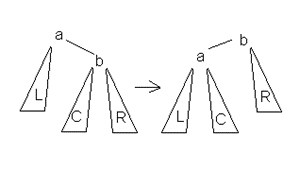
\includegraphics[width=0.6\textwidth]{media/image8.png}
    \end{figure}
    
    \item Большое левое вращение
    \begin{figure}[H]
        \centering
        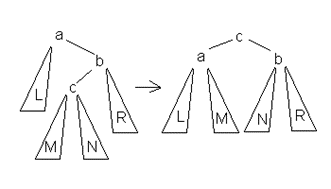
\includegraphics[width=0.7\textwidth]{media/image9.png}
    \end{figure}
    
    \item Малое правое вращение
    \begin{figure}[H]
        \centering
        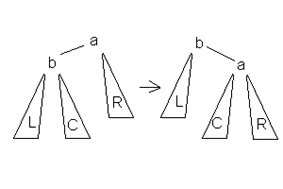
\includegraphics[width=0.6\textwidth]{media/image10.png}
    \end{figure}
    
    \item Большое правое вращение
    \begin{figure}[H]
        \centering
        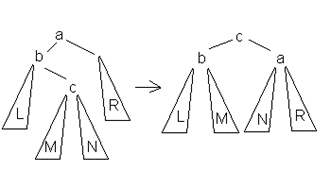
\includegraphics[width=0.7\textwidth]{media/image11.png}
    \end{figure}
\end{itemize}

\subsubsection{Красно-чёрное дерево (Red-black tree)}
\label{subsubsec:красно-чёрное-дерево-red-black-tree}

Красно-чёрное дерево --- это самобалансирующееся двоичное дерево поиска, которое гарантирует логарифмическую высоту дерева при любых последовательностях операций. Балансировка достигается за счёт использования дополнительного цвета (красный/чёрный) для каждого узла и соблюдения набора свойств: 1) Каждый узел либо красный, либо чёрный. 2) Корень всегда чёрный. 3) Все листья (NIL) чёрные. 4) У красного узла оба потомка чёрные. 5) Все пути от узла до листьев содержат одинаковое количество чёрных узлов.

\begin{table}[H]
    \centering
    \begin{tabular}{|l|c|c|c|}
        \hline
        Операция & Лучший случай & Средний случай & Худший случай \\
        \hline
        Вставка элемента & $O(1)$ & $O(\log(n))$ & $O(\log(n))$ \\
        \hline
        Удаление элемента & $O(1)$ & $O(\log(n))$ & $O(\log(n))$ \\
        \hline
        Поиск элемента & $O(1)$ & $O(\log(n))$ & $O(\log(n))$ \\
        \hline
        \makecell[l]{Вычисление высоты \\дерева} & $O(\log(n))$ & $O(\log(n))$ & $O(\log(n))$ \\
        \hline
    \end{tabular}
    \caption{Сложность операций для красно-чёрного дерева}
\end{table}

Для балансировки красно-чёрного дерева есть следующие операции:

\begin{itemize}
    \item Левый поворот
    \item Правый поворот
    \item Перекрашивание узлов
\end{itemize}

\subsubsection{Дерево отрезков (Segment tree)}
\label{subsubsec:дерево-отрезков-segment-tree}

Дерево отрезков --- это древовидная структура данных, которая позволяет эффективно выполнять операции на отрезках массива (диапазонах элементов). Она предварительно вычисляет и хранит агрегированную информацию об отрезках, что позволяет быстро отвечать на запросы.

\begin{table}[H]
    \centering
    \begin{tabular}{|l|c|c|c|}
        \hline
        Операция & Лучший случай & Средний случай & Худший случай \\
        \hline
        Вставка элемента & $O(n)$ & $O(n)$ & $O(n)$ \\
        \hline
        Удаление элемента & $O(n)$ & $O(n)$ & $O(n)$ \\
        \hline
        Обновление элемента & $O(1)$ & $O(\log(n))$ & $O(\log(n))$ \\
        \hline
        Поиск элемента & $O(n)$ & $O(n)$ & $O(n)$ \\
        \hline
        \makecell[l]{Вычисление высоты \\дерева} & $O(1)$ & $O(1)$ & $O(1)$ \\
        \hline
    \end{tabular}
    \caption{Сложность операций для дерева отрезков}
\end{table}

\subsubsection{B-дерево (B-tree)}
\label{subsubsec:b-дерево-b-tree}

B-дерево --- это сбалансированное дерево поиска. Каждый узел может содержать множество ключей (кроме корня) и иметь много потомков, что минимизирует высоту дерева. Также в B-дереве все листья находятся на одном уровне.

\begin{table}[H]
    \centering
    \begin{tabular}{|l|c|c|c|}
        \hline
        Операция & Лучший случай & Средний случай & Худший случай \\
        \hline
        Вставка элемента & $O(1)$ & $O(\log(n))$ & $O(\log(n))$ \\
        \hline
        Удаление элемента & $O(1)$ & $O(\log(n))$ & $O(\log(n))$ \\
        \hline
        Поиск элемента & $O(1)$ & $O(\log(n))$ & $O(\log(n))$ \\
        \hline
        \makecell[l]{Вычисление высоты \\дерева} & $O(1)$ & $O(\log(n))$ & $O(\log(n))$ \\
        \hline
    \end{tabular}
    \caption{Сложность операций для B-дерева}
\end{table}

\subsubsection{B+-дерево (B+-tree)}
\label{subsubsec:b-дерево-b-tree-1}

B+-дерево --- это вариант B-дерева, где все данные хранятся только в листьях, а внутренние узлы содержат только ключи-указатели. Это делает структуру особенно эффективной для диапазонных запросов и последовательного доступа. Также в B+-дереве все листья связанны между собой и образуют связанный список.

\begin{table}[H]
    \centering
    \begin{tabular}{|l|c|c|c|}
        \hline
        Операция & Лучший случай & Средний случай & Худший случай \\
        \hline
        Вставка элемента & $O(1)$ & $O(\log(n))$ & $O(\log(n))$ \\
        \hline
        Удаление элемента & $O(1)$ & $O(\log(n))$ & $O(\log(n))$ \\
        \hline
        Поиск элемента & $O(1)$ & $O(\log(n))$ & $O(\log(n))$ \\
        \hline
        \makecell[l]{Диапазонный запрос \\с $k$ элементами} & $O(1)$ & $O(k + \log(n))$ & $O(k + \log(n))$ \\
        \hline
        \makecell[l]{Вычисление высоты \\дерева} & $O(1)$ & $O(\log(n))$ & $O(\log(n))$ \\
        \hline
    \end{tabular}
    \caption{Сложность операций для B+-дерева}
\end{table}

\subsubsection{Куча (Heap)}
\label{subsubsec:куча-heap}

Куча --- это специализированная древовидная структура данных, которая удовлетворяет свойству кучи: каждый родитель больше своих потомков для максимальной кучи или каждый родитель меньше своих потомков для минимальной кучи. Это позволяет эффективно находить и извлекать элемент с наивысшим (или наименьшим) приоритетом.

\begin{table}[H]
    \centering
    \begin{tabular}{|l|c|c|c|}
        \hline
        Операция & Лучший случай & Средний случай & Худший случай \\
        \hline
        Вставка элемента & $O(1)$ & $O(\log(n))$ & $O(\log(n))$ \\
        \hline
        Удаление элемента & $O(\log(n))$ & $O(\log(n))$ & $O(\log(n))$ \\
        \hline
        Поиск элемента & $O(1)$ & $O(n)$ & $O(n)$ \\
        \hline
        Изменение приоритета & $O(1)$ & $O(n)$ & $O(n)$ \\
        \hline
    \end{tabular}
    \caption{Сложность операций для кучи}
\end{table}

\subsubsection{Двоичная куча (Binary heap)}
\label{subsubsec:двоичная-куча-binary-heap}

Двоичная куча --- это частный случай обычной кучи, когда каждый узел имеет не более двух потомков.

\subsubsection{Префиксное дерево (Trie)}
\label{subsubsec:префиксное-дерево-trie}

Префиксное дерево --- это древовидная структура данных для эффективного хранения и поиска строк. Ключи обычно являются строками, а узлы хранят символы и ссылки на следующие символы, образуя пути от корня до листьев, соответствующие строкам.

\begin{table}[H]
    \centering
    \begin{tabular}{|l|c|c|c|}
        \hline
        Операция & Лучший случай & Средний случай & Худший случай \\
        \hline
        Вставка слова длины $m$ & $O(1)$ & $O(m)$ & $O(m)$ \\
        \hline
        Удаление слова длины $m$ & $O(1)$ & $O(m)$ & $O(m)$ \\
        \hline
        Поиск слова длины $m$ & $O(1)$ & $O(m)$ & $O(m)$ \\
        \hline
        \makecell[l]{Авто дополнение $k$ слов \\с префиксом длины $m$} & $O(1)$ & $O(k + m)$ & $O(k + m)$ \\
        \hline
        Поиск всех слов & $O(1)$ & $O(n)$ & $O(n)$ \\
        \hline
    \end{tabular}
    \caption{Сложность операций для префиксного дерева}
\end{table}

\subsubsection{Декартово дерево (Treap/Cartesian tree)}
\label{subsubsec:декартово-дерево-treapcartesian-tree}

Декартово дерево --- это структура данных, сочетающая в себе свойства бинарного дерева поиска и кучи. Каждый узел содержит два ключа: один используется для упорядочивания как в бинарном дереве поиска, а другой --- как в куче.

\begin{table}[H]
    \centering
    \begin{tabular}{|l|c|c|c|}
        \hline
        Операция & Лучший случай & Средний случай & Худший случай \\
        \hline
        Вставка элемента & $O(1)$ & $O(\log(n))$ & $O(n)$ \\
        \hline
        Удаление элемента & $O(1)$ & $O(\log(n))$ & $O(n)$ \\
        \hline
        Поиск элемента & $O(1)$ & $O(\log(n))$ & $O(n)$ \\
        \hline
        \makecell[l]{Объединение двух \\деревьев} & $O(1)$ & $O(\log(n))$ & $O(n)$ \\
        \hline
        Разделение дерева & $O(1)$ & $O(\log(n))$ & $O(n)$ \\
        \hline
    \end{tabular}
    \caption{Сложность операций для декартова дерева}
\end{table}

\subsubsection{Splay-дерево (Splay tree)}
\label{subsubsec:splay-дерево-splay-tree}

Splay-дерево --- это самобалансирующееся бинарное дерево поиска, которое выполняет операцию «splay» (перемещение) для элемента, к которому был выполнен доступ, перемещая его в корень дерева. Это позволяет часто используемым элементам быть ближе к корню.

\begin{table}[H]
    \centering
    \begin{tabular}{|l|c|c|c|}
        \hline
        Операция & Лучший случай & Средний случай & Худший случай \\
        \hline
        Вставка элемента & $O(1)$ & $O(\log(n))$ & $O(n)$ \\
        \hline
        Удаление элемента & $O(1)$ & $O(\log(n))$ & $O(n)$ \\
        \hline
        Поиск элемента & $O(1)$ & $O(\log(n))$ & $O(n)$ \\
        \hline
        Доступ к элементу & $O(1)$ & $O(\log(n))$ & $O(n)$ \\
        \hline
    \end{tabular}
    \caption{Сложность операций для Splay-дерева}
\end{table}

\subsubsection{Дерево квадрантов (Quadtree)}
\label{subsubsec:дерево-квадрантов-quadtree}

Дерево квадрантов --- это древовидная структура данных, в которой каждый внутренний узел имеет ровно четыре потомка. Используется для разбиения двумерного пространства путем рекурсивного деления его на четыре квадранта.

\begin{table}[H]
    \centering
    \begin{tabular}{|l|c|c|c|}
        \hline
        Операция & Лучший случай & Средний случай & Худший случай \\
        \hline
        Вставка точки & $O(1)$ & $O(\log(n))$ & $O(n)$ \\
        \hline
        Удаление точки & $O(1)$ & $O(\log(n))$ & $O(n)$ \\
        \hline
        Поиск точки & $O(1)$ & $O(\log(n))$ & $O(n)$ \\
        \hline
        Поиск в области & $O(1)$ & $O(\sqrt{n} + k)$ & $O(n)$ \\
        \hline
    \end{tabular}
    \caption{Сложность операций для дерева квадрантов}
\end{table}

\subsubsection{Дерево восьмеричных разбиений (Octree)}
\label{subsubsec:дерево-восьмеричных-разбиений-octree}

Дерево восьмеричных разбиений --- это древовидная структура данных, в которой каждый внутренний узел имеет ровно восемь потомков. Используется для разбиения трехмерного пространства путем рекурсивного деления его на восемь октантов.

\begin{table}[H]
    \centering
    \begin{tabular}{|l|c|c|c|}
        \hline
        Операция & Лучший случай & Средний случай & Худший случай \\
        \hline
        Вставка точки & $O(1)$ & $O(\log(n))$ & $O(n)$ \\
        \hline
        Удаление точки & $O(1)$ & $O(\log(n))$ & $O(n)$ \\
        \hline
        Поиск точки & $O(1)$ & $O(\log(n))$ & $O(n)$ \\
        \hline
        Поиск в объеме & $O(1)$ & $O(\sqrt[3]{n} + k)$ & $O(n)$ \\
        \hline
    \end{tabular}
    \caption{Сложность операций для дерева восьмеричных разбиений}
\end{table}

\subsubsection{Арифметическое дерево выражения (Expression tree)}
\label{subsubsec:арифметическое-дерево-выражения-expression-tree}

Арифметическое дерево выражения --- это бинарное дерево, используемое для представления арифметических выражений. Листья дерева представляют операнды, а внутренние узлы --- операторы.

\begin{table}[H]
    \centering
    \begin{tabular}{|l|c|c|c|}
        \hline
        Операция & Лучший случай & Средний случай & Худший случай \\
        \hline
        Построение дерева & $O(n)$ & $O(n)$ & $O(n)$ \\
        \hline
        Вычисление выражения & $O(1)$ & $O(n)$ & $O(n)$ \\
        \hline
        Обход дерева & $O(1)$ & $O(n)$ & $O(n)$ \\
        \hline
        Оптимизация дерева & $O(1)$ & $O(n)$ & $O(n^2)$ \\
        \hline
    \end{tabular}
    \caption{Сложность операций для арифметического дерева выражения}
\end{table}

\subsubsection{Неориентированный граф (Undirected graph)}
\label{subsubsec:неориентированный-граф-undirected-graph}

Неориентированный граф --- это граф, в котором рёбра не имеют направления. Связь между вершинами является двусторонней.

\begin{table}[H]
    \centering
    \begin{tabular}{|l|c|c|c|}
        \hline
        Операция & Лучший случай & Средний случай & Худший случай \\
        \hline
        Добавление вершины & $O(1)$ & $O(1)$ & $O(1)$ \\
        \hline
        Добавление ребра & $O(1)$ & $O(1)$ & $O(1)$ \\
        \hline
        Удаление вершины & $O(1)$ & $O(deg(v))$ & $O(n)$ \\
        \hline
        Удаление ребра & $O(1)$ & $O(1)$ & $O(1)$ \\
        \hline
        Поиск соседей & $O(1)$ & $O(deg(v))$ & $O(n)$ \\
        \hline
        Проверка смежности & $O(1)$ & $O(deg(v))$ & $O(n)$ \\
        \hline
    \end{tabular}
    \caption{Сложность операций для неориентированного графа}
\end{table}

\subsubsection{Ориентированный граф (Directed graph/Digraph)}
\label{subsubsec:ориентированный-граф-directed-graphdigraph}

Ориентированный граф --- это граф, в котором рёбра имеют направление. Связь между вершинами является односторонней.

\begin{table}[H]
    \centering
    \begin{tabular}{|l|c|c|c|}
        \hline
        Операция & Лучший случай & Средний случай & Худший случай \\
        \hline
        Добавление вершины & $O(1)$ & $O(1)$ & $O(1)$ \\
        \hline
        Добавление ребра & $O(1)$ & $O(1)$ & $O(1)$ \\
        \hline
        Удаление вершины & $O(1)$ & $O(deg^+(v) + deg^-(v))$ & $O(n)$ \\
        \hline
        Удаление ребра & $O(1)$ & $O(1)$ & $O(1)$ \\
        \hline
        \makecell[l]{Поиск исходящих \\соседей} & $O(1)$ & $O(deg^+(v))$ & $O(n)$ \\
        \hline
        \makecell[l]{Поиск входящих \\соседей} & $O(1)$ & $O(deg^-(v))$ & $O(n)$ \\
        \hline
    \end{tabular}
    \caption{Сложность операций для ориентированного графа}
\end{table}

\subsubsection{Взвешенный граф (Weighted graph)}
\label{subsubsec:взвешенный-граф-weighted-graph}

Взвешенный граф --- это граф, в котором каждому ребру присвоен числовой вес (стоимость, длина и т.д.).

\begin{table}[H]
    \centering
    \begin{tabular}{|l|c|c|c|}
        \hline
        Операция & Лучший случай & Средний случай & Худший случай \\
        \hline
        Добавление ребра с весом & $O(1)$ & $O(1)$ & $O(1)$ \\
        \hline
        Изменение веса ребра & $O(1)$ & $O(1)$ & $O(1)$ \\
        \hline
        Поиск минимального пути & $O(1)$ & $O(n \log n + m)$ & $O(n \log n + m)$ \\
        \hline
        \makecell[l]{Поиск минимального \\остовного дерева} & $O(1)$ & $O(m \log n)$ & $O(m \log n)$ \\
        \hline
    \end{tabular}
    \caption{Сложность операций для взвешенного графа}
\end{table}

\subsubsection{Граф с метками (Labeled graph)}
\label{subsubsec:граф-с-метками-labeled-graph}

Граф с метками --- это граф, в котором вершины и/или рёбра имеют метки (названия, категории и т.д.).

\begin{table}[H]
    \centering
    \begin{tabular}{|l|c|c|c|}
        \hline
        Операция & Лучший случай & Средний случай & Худший случай \\
        \hline
        Поиск по метке вершины & $O(1)$ & $O(n)$ & $O(n)$ \\
        \hline
        Поиск по метке ребра & $O(1)$ & $O(m)$ & $O(m)$ \\
        \hline
        Изменение метки & $O(1)$ & $O(1)$ & $O(1)$ \\
        \hline
        Группировка по меткам & $O(1)$ & $O(n + m)$ & $O(n + m)$ \\
        \hline
    \end{tabular}
    \caption{Сложность операций для графа с метками}
\end{table}

\subsubsection{Лес (Forest)}
\label{subsubsec:лес-forest}

Лес --- это множество непересекающихся деревьев, или ациклический неориентированный граф.

\begin{table}[H]
    \centering
    \begin{tabular}{|l|c|c|c|}
        \hline
        Операция & Лучший случай & Средний случай & Худший случай \\
        \hline
        Добавление дерева & $O(1)$ & $O(1)$ & $O(1)$ \\
        \hline
        Объединение деревьев & $O(1)$ & $O(n)$ & $O(n)$ \\
        \hline
        \makecell[l]{Поиск компоненты \\связности} & $O(1)$ & $O(\alpha(n))$ & $O(\alpha(n))$ \\
        \hline
        Подсчет деревьев & $O(1)$ & $O(1)$ & $O(1)$ \\
        \hline
    \end{tabular}
    \caption{Сложность операций для леса}
\end{table}

\subsubsection{Связный граф (Connected graph)}
\label{subsubsec:связный-граф-connected-graph}

Связный граф --- это граф, в котором существует путь между любой парой вершин.

\begin{table}[H]
    \centering
    \begin{tabular}{|l|c|c|c|}
        \hline
        Операция & Лучший случай & Средний случай & Худший случай \\
        \hline
        Проверка связности & $O(1)$ & $O(n + m)$ & $O(n + m)$ \\
        \hline
        \makecell[l]{Поиск компонент \\связности} & $O(1)$ & $O(n + m)$ & $O(n + m)$ \\
        \hline
        Поиск мостов & $O(1)$ & $O(n + m)$ & $O(n + m)$ \\
        \hline
        Поиск точек сочленения & $O(1)$ & $O(n + m)$ & $O(n + m)$ \\
        \hline
    \end{tabular}
    \caption{Сложность операций для связного графа}
\end{table}

\subsubsection{Полный граф (Complete graph)}
\label{subsubsec:полный-граф-complete-graph}

Полный граф --- это граф, в котором каждая пара различных вершин соединена ребром.

\begin{table}[H]
    \centering
    \begin{tabular}{|l|c|c|c|}
        \hline
        Операция & Лучший случай & Средний случай & Худший случай \\
        \hline
        Добавление вершины & $O(n)$ & $O(n)$ & $O(n)$ \\
        \hline
        Удаление вершины & $O(n)$ & $O(n)$ & $O(n)$ \\
        \hline
        Проверка смежности & $O(1)$ & $O(1)$ & $O(1)$ \\
        \hline
        Подсчет ребер & $O(1)$ & $O(1)$ & $O(1)$ \\
        \hline
    \end{tabular}
    \caption{Сложность операций для полного графа}
\end{table}

\subsubsection{Двудольный граф (Bipartite graph)}
\label{subsubsec:двудольный-граф-bipartite-graph}

Двудольный граф --- это граф, вершины которого можно разбить на два непересекающихся множества так, что каждое ребро соединяет вершины из разных множеств.

\begin{table}[H]
    \centering
    \begin{tabular}{|l|c|c|c|}
        \hline
        Операция & Лучший случай & Средний случай & Худший случай \\
        \hline
        Проверка двудольности & $O(1)$ & $O(n + m)$ & $O(n + m)$ \\
        \hline
        \makecell[l]{Поиск максимального \\паросочетания} & $O(1)$ & $O(m \sqrt{n})$ & $O(m \sqrt{n})$ \\
        \hline
        Разбиение на доли & $O(1)$ & $O(n + m)$ & $O(n + m)$ \\
        \hline
        \makecell[l]{Проверка полной \\двудольности} & $O(1)$ & $O(n + m)$ & $O(n + m)$ \\
        \hline
    \end{tabular}
    \caption{Сложность операций для двудольного графа}
\end{table}

\subsubsection{Ациклический ориентированный граф (Directed acyclic graph --- DAG)}
\label{subsubsec:ациклический-ориентированный-граф-directed-acyclic-graph-dag}

Ациклический ориентированный граф --- это ориентированный граф без направленных циклов. Широко используется для представления структур с зависимостями.

\begin{table}[H]
    \centering
    \begin{tabular}{|l|c|c|c|}
        \hline
        Операция & Лучший случай & Средний случай & Худший случай \\
        \hline
        \makecell[l]{Топологическая \\сортировка} & $O(1)$ & $O(n + m)$ & $O(n + m)$ \\
        \hline
        \makecell[l]{Поиск критического \\пути} & $O(1)$ & $O(n + m)$ & $O(n + m)$ \\
        \hline
        Проверка достижимости & $O(1)$ & $O(n + m)$ & $O(n + m)$ \\
        \hline
        \makecell[l]{Поиск транзитивного \\замыкания} & $O(1)$ & $O(n^2)$ & $O(n^2)$ \\
        \hline
    \end{tabular}
    \caption{Сложность операций для ациклического ориентированного графа}
\end{table}

\subsubsection{Матрица (Matrix)}
\label{subsubsec:матрица-matrix}

Матрица --- это двумерная структура данных, состоящая из строк и столбцов. Каждый элемент матрицы имеет два индекса: номер строки и номер столбца.

\begin{table}[H]
    \centering
    \begin{tabular}{|l|c|c|c|}
        \hline
        Операция & Лучший случай & Средний случай & Худший случай \\
        \hline
        Доступ к элементу & $O(1)$ & $O(1)$ & $O(1)$ \\
        \hline
        Изменение элемента & $O(1)$ & $O(1)$ & $O(1)$ \\
        \hline
        Транспонирование & $O(1)$ & $O(n \cdot m)$ & $O(n \cdot m)$ \\
        \hline
        Сложение матриц & $O(1)$ & $O(n \cdot m)$ & $O(n \cdot m)$ \\
        \hline
        Умножение матриц & $O(1)$ & $O(n \cdot m \cdot k)$ & $O(n \cdot m \cdot k)$ \\
        \hline
    \end{tabular}
    \caption{Сложность операций для матрицы}
\end{table}

\subsubsection{Тензор (Tensor)}
\label{subsubsec:тензор-tensor}

Тензор --- это многомерная структура данных, обобщающая понятия скаляра (0-мерный тензор), вектора (1-мерный тензор) и матрицы (2-мерный тензор). Тензоры могут иметь произвольное количество измерений.

\begin{table}[H]
    \centering
    \begin{tabular}{|l|c|c|c|}
        \hline
        Операция & Лучший случай & Средний случай & Худший случай \\
        \hline
        Доступ к элементу & $O(1)$ & $O(1)$ & $O(1)$ \\
        \hline
        Изменение элемента & $O(1)$ & $O(1)$ & $O(1)$ \\
        \hline
        Сложение тензоров & $O(1)$ & $O(\prod d_i)$ & $O(\prod d_i)$ \\
        \hline
        Тензорное произведение & $O(1)$ & $O(\prod d_i \cdot \prod e_j)$ & $O(\prod d_i \cdot \prod e_j)$ \\
        \hline
        Свертка & $O(1)$ & $O(\prod d_i)$ & $O(\prod d_i)$ \\
        \hline
    \end{tabular}
    \caption{Сложность операций для тензора}
\end{table}

\section{Алгоритмы}
\label{sec:универсальные-алгоритмы}

Алгоритм --- это конечная последовательность четко определенных инструкций, предназначенная для решения конкретной задачи или класса задач. Алгоритмы являются фундаментальным понятием в информатике и лежат в основе всех компьютерных программ.

Ключевые характеристики алгоритмов:

\begin{itemize}
    \item Конечность: алгоритм должен завершаться после выполнения конечного числа шагов.
    \item Определенность: каждая инструкция должна быть четкой и однозначной.
    \item Входные данные: алгоритм принимает ноль или более входных значений.
    \item Выходные данные: алгоритм производит один или более результатов.
    \item Эффективность: алгоритм должен использовать разумное количество ресурсов (время, память).
\end{itemize}

\subsection{Алгоритмы сортировки}
\label{subsec:алгоритмы-сортировки}

Алгоритмы сортировки предназначены для упорядочивания элементов в структуре данных согласно определенному критерию (обычно по возрастанию или убыванию). Выбор алгоритма сортировки зависит от размера данных, их частичной упорядоченности и требований к стабильности.

\subsubsection{Сортировка пузырьком (Bubble sort)}
\label{subsubsec:сортировка-пузырьком-bubble-sort}

Сортировка пузырьком --- это простой алгоритм сортировки, который многократно проходит по массиву, сравнивает соседние элементы и меняет их местами, если они находятся в неправильном порядке. Проходы повторяются до тех пор, пока массив не будет отсортирован.

\begin{table}[H]
    \centering
    \begin{tabular}{|l|c|c|c|}
        \hline
        Случай & Лучший & Средний & Худший \\
        \hline
        Временная сложность & $O(n)$ & $O(n^2)$ & $O(n^2)$ \\
        \hline
        Пространственная сложность & $O(1)$ & $O(1)$ & $O(1)$ \\
        \hline
        Стабильность & Да & Да & Да \\
        \hline
        Адаптивность & Да & Нет & Нет \\
        \hline
    \end{tabular}
    \caption{Характеристики сортировки пузырьком}
\end{table}

\subsubsection{Сортировка выбором (Selection sort)}
\label{subsubsec:сортировка-выбором-selection-sort}

Сортировка выбором --- это алгоритм, который на каждом проходе находит минимальный (или максимальный) элемент в неотсортированной части массива и помещает его в конец отсортированной части.

\begin{table}[H]
    \centering
    \begin{tabular}{|l|c|c|c|}
        \hline
        Случай & Лучший & Средний & Худший \\
        \hline
        Временная сложность & $O(n^2)$ & $O(n^2)$ & $O(n^2)$ \\
        \hline
        Пространственная сложность & $O(1)$ & $O(1)$ & $O(1)$ \\
        \hline
        Стабильность & Нет & Нет & Нет \\
        \hline
        Адаптивность & Нет & Нет & Нет \\
        \hline
    \end{tabular}
    \caption{Характеристики сортировки выбором}
\end{table}

\subsubsection{Сортировка вставками (Insertion sort)}
\label{subsubsec:сортировка-вставками-insertion-sort}

Сортировка вставками --- это алгоритм, который строит отсортированную последовательность постепенно, вставляя каждый следующий элемент в правильную позицию среди уже отсортированных элементов.

\begin{table}[H]
    \centering
    \begin{tabular}{|l|c|c|c|}
        \hline
        Случай & Лучший & Средний & Худший \\
        \hline
        Временная сложность & $O(n)$ & $O(n^2)$ & $O(n^2)$ \\
        \hline
        Пространственная сложность & $O(1)$ & $O(1)$ & $O(1)$ \\
        \hline
        Стабильность & Да & Да & Да \\
        \hline
        Адаптивность & Да & Нет & Нет \\
        \hline
    \end{tabular}
    \caption{Характеристики сортировки вставками}
\end{table}

\subsubsection{Сортировка слиянием (Merge sort)}
\label{subsubsec:сортировка-слиянием-merge-sort}

Сортировка слиянием --- это алгоритм «разделяй и властвуй», который рекурсивно разбивает массив на две половины, сортирует их, а затем объединяет отсортированные половины в один отсортированный массив.

\begin{table}[H]
    \centering
    \begin{tabular}{|l|c|c|c|}
        \hline
        Случай & Лучший & Средний & Худший \\
        \hline
        Временная сложность & $O(n \log n)$ & $O(n \log n)$ & $O(n \log n)$ \\
        \hline
        Пространственная сложность & $O(n)$ & $O(n)$ & $O(n)$ \\
        \hline
        Стабильность & Да & Да & Да \\
        \hline
        Адаптивность & Нет & Нет & Нет \\
        \hline
    \end{tabular}
    \caption{Характеристики сортировки слиянием}
\end{table}

\subsubsection{Быстрая сортировка (Quick sort)}
\label{subsubsec:быстрая-сортировка-quick-sort}

Быстрая сортировка --- это алгоритм «разделяй и властвуй», который выбирает опорный элемент, разбивает массив на две части (элементы меньше опорного и элементы больше опорного), а затем рекурсивно сортирует эти части.

\begin{table}[H]
    \centering
    \begin{tabular}{|l|c|c|c|}
        \hline
        Случай & Лучший & Средний & Худший \\
        \hline
        Временная сложность & $O(n \log n)$ & $O(n \log n)$ & $O(n^2)$ \\
        \hline
        Пространственная сложность & $O(\log n)$ & $O(\log n)$ & $O(n)$ \\
        \hline
        Стабильность & Нет & Нет & Нет \\
        \hline
        Адаптивность & Нет & Нет & Нет \\
        \hline
    \end{tabular}
    \caption{Характеристики быстрой сортировки}
\end{table}

\subsubsection{Пирамидальная сортировка (Heap sort)}
\label{subsubsec:пирамидальная-сортировка-heap-sort}

Пирамидальная сортировка --- это алгоритм, который использует структуру данных «куча» для сортировки элементов. Алгоритм строит max-кучу из массива, затем многократно извлекает максимальный элемент и перестраивает кучу.

\begin{table}[H]
    \centering
    \begin{tabular}{|l|c|c|c|}
        \hline
        Случай & Лучший & Средний & Худший \\
        \hline
        Временная сложность & $O(n \log n)$ & $O(n \log n)$ & $O(n \log n)$ \\
        \hline
        Пространственная сложность & $O(1)$ & $O(1)$ & $O(1)$ \\
        \hline
        Стабильность & Нет & Нет & Нет \\
        \hline
        Адаптивность & Нет & Нет & Нет \\
        \hline
    \end{tabular}
    \caption{Характеристики пирамидальной сортировки}
\end{table}

\subsubsection{Сортировка Шелла (Shell sort)}
\label{subsubsec:сортировка-шелла-shell-sort}

Сортировка Шелла --- это алгоритм, который является обобщением сортировки вставками. Он сортирует элементы, находящиеся на определенном расстоянии друг от друга, постепенно уменьшая это расстояние.

\begin{table}[H]
    \centering
    \begin{tabular}{|l|c|c|c|}
        \hline
        Случай & Лучший & Средний & Худший \\
        \hline
        Временная сложность & $O(n \log n)$ & $O(n^{1.5})$ & $O(n^2)$ \\
        \hline
        Пространственная сложность & $O(1)$ & $O(1)$ & $O(1)$ \\
        \hline
        Стабильность & Нет & Нет & Нет \\
        \hline
        Адаптивность & Да & Нет & Нет \\
        \hline
    \end{tabular}
    \caption{Характеристики сортировки Шелла}
\end{table}

\subsubsection{Сортировка деревом (Tree sort)}
\label{subsubsec:сортировка-деревом-tree-sort}

Сортировка деревом --- это алгоритм, который использует бинарное дерево поиска для сортировки элементов. Элементы вставляются в дерево, а затем обходом в порядке возрастания извлекаются в отсортированном виде.

\begin{table}[H]
    \centering
    \begin{tabular}{|l|c|c|c|}
        \hline
        Случай & Лучший & Средний & Худший \\
        \hline
        Временная сложность & $O(n \log n)$ & $O(n \log n)$ & $O(n^2)$ \\
        \hline
        Пространственная сложность & $O(n)$ & $O(n)$ & $O(n)$ \\
        \hline
        Стабильность & Да & Да & Да \\
        \hline
        Адаптивность & Нет & Нет & Нет \\
        \hline
    \end{tabular}
    \caption{Характеристики сортировки деревом}
\end{table}

\subsubsection{Сортировка подсчётом (Counting sort)}
\label{subsubsec:сортировка-подсчётом-counting-sort}

Сортировка подсчётом --- это алгоритм, который работает путем подсчета количества элементов с каждым distinct значением, а затем использует эту информацию для определения позиций элементов в отсортированной последовательности. Эффективен, когда диапазон значений ограничен.

\begin{table}[H]
    \centering
    \begin{tabular}{|l|c|c|c|}
        \hline
        Случай & Лучший & Средний & Худший \\
        \hline
        Временная сложность & $O(n + k)$ & $O(n + k)$ & $O(n + k)$ \\
        \hline
        Пространственная сложность & $O(k)$ & $O(k)$ & $O(k)$ \\
        \hline
        Стабильность & Да & Да & Да \\
        \hline
        Адаптивность & Нет & Нет & Нет \\
        \hline
    \end{tabular}
    \caption{Характеристики сортировки подсчётом}
\end{table}

\subsubsection{Поразрядная сортировка (Radix sort)}
\label{subsubsec:поразрядная-сортировка-radix-sort}

Поразрядная сортировка --- это алгоритм, который сортирует числа поразрядно, начиная с младшего разряда и заканчивая старшим. Для сортировки каждого разряда обычно используется стабильный алгоритм сортировки (часто сортировка подсчётом).

\begin{table}[H]
    \centering
    \begin{tabular}{|l|c|c|c|}
        \hline
        Случай & Лучший & Средний & Худший \\
        \hline
        Временная сложность & $O(nk)$ & $O(nk)$ & $O(nk)$ \\
        \hline
        Пространственная сложность & $O(n + k)$ & $O(n + k)$ & $O(n + k)$ \\
        \hline
        Стабильность & Да & Да & Да \\
        \hline
        Адаптивность & Нет & Нет & Нет \\
        \hline
    \end{tabular}
    \caption{Характеристики поразрядной сортировки}
\end{table}

\subsubsection{Блочная/Карманная сортировка (Bucket sort)}
\label{subsubsec:блочная-карманная-сортировка-bucket-sort}

Блочная сортировка --- это алгоритм, который распределяет элементы по «ведрам» (блокам), затем сортирует каждое ведро отдельно и объединяет результаты.

\begin{table}[H]
    \centering
    \begin{tabular}{|l|c|c|c|}
        \hline
        Случай & Лучший & Средний & Худший \\
        \hline
        Временная сложность & $O(n + k)$ & $O(n + k)$ & $O(n^2)$ \\
        \hline
        Пространственная сложность & $O(n + k)$ & $O(n + k)$ & $O(n + k)$ \\
        \hline
        Стабильность & Да & Да & Да \\
        \hline
        Адаптивность & Нет & Нет & Нет \\
        \hline
    \end{tabular}
    \caption{Характеристики блочной сортировки}
\end{table}

\subsubsection{Тимо-сортировка (Tim sort)}
\label{subsubsec:тимо-сортировка-tim-sort}

Тимо-сортировка --- это гибридный алгоритм, сочетающий сортировку вставками и слиянием. Оптимизирован для работы с реальными данными, часто содержащими упорядоченные подпоследовательности.

\begin{table}[H]
    \centering
    \begin{tabular}{|l|c|c|c|}
        \hline
        Случай & Лучший & Средний & Худший \\
        \hline
        Временная сложность & $O(n)$ & $O(n \log n)$ & $O(n \log n)$ \\
        \hline
        Пространственная сложность & $O(n)$ & $O(n)$ & $O(n)$ \\
        \hline
        Стабильность & Да & Да & Да \\
        \hline
        Адаптивность & Да & Да & Да \\
        \hline
    \end{tabular}
    \caption{Характеристики Тимо-сортировки}
\end{table}

\subsubsection{Интроспективная сортировка (Introspective sort)}
\label{subsubsec:интроспективная-сортировка-introspective-sort}

Интроспективная сортировка --- это гибридный алгоритм, который начинает как быстрая сортировка, но переключается на пирамидальную сортировку, если глубина рекурсии становится слишком большой.

\begin{table}[H]
    \centering
    \begin{tabular}{|l|c|c|c|}
        \hline
        Случай & Лучший & Средний & Худший \\
        \hline
        Временная сложность & $O(n \log n)$ & $O(n \log n)$ & $O(n \log n)$ \\
        \hline
        Пространственная сложность & $O(\log n)$ & $O(\log n)$ & $O(\log n)$ \\
        \hline
        Стабильность & Нет & Нет & Нет \\
        \hline
        Адаптивность & Нет & Нет & Нет \\
        \hline
    \end{tabular}
    \caption{Характеристики интроспективной сортировки}
\end{table}

\subsubsection{Гномья сортировка (Gnome sort)}
\label{subsubsec:гномья-сортировка-gnome-sort}

Гномья сортировка --- это простой алгоритм, похожий на сортировку вставками, но работающий путем попарного сравнения и обмена соседних элементов.

\begin{table}[H]
    \centering
    \begin{tabular}{|l|c|c|c|}
        \hline
        Случай & Лучший & Средний & Худший \\
        \hline
        Временная сложность & $O(n)$ & $O(n^2)$ & $O(n^2)$ \\
        \hline
        Пространственная сложность & $O(1)$ & $O(1)$ & $O(1)$ \\
        \hline
        Стабильность & Да & Да & Да \\
        \hline
        Адаптивность & Да & Нет & Нет \\
        \hline
    \end{tabular}
    \caption{Характеристики гномьей сортировки}
\end{table}

\subsubsection{Сортировка расчёской (Comb sort)}
\label{subsubsec:сортировка-расчёской-comb-sort}

Сортировка расчёской --- это улучшение сортировки пузырьком, которое использует увеличивающийся промежуток между сравниваемыми элементами.

\begin{table}[H]
    \centering
    \begin{tabular}{|l|c|c|c|}
        \hline
        Случай & Лучший & Средний & Худший \\
        \hline
        Временная сложность & $O(n \log n)$ & $O(n^2)$ & $O(n^2)$ \\
        \hline
        Пространственная сложность & $O(1)$ & $O(1)$ & $O(1)$ \\
        \hline
        Стабильность & Нет & Нет & Нет \\
        \hline
        Адаптивность & Да & Нет & Нет \\
        \hline
    \end{tabular}
    \caption{Характеристики сортировки расчёской}
\end{table}

\subsubsection{Глупая сортировка (Bogo sort)}
\label{subsubsec:глупая-сортировка-bogo-sort}

Глупая сортировка --- это неэффективный алгоритм, который случайным образом переставляет элементы до тех пор, пока массив не окажется отсортированным.

\begin{table}[H]
    \centering
    \begin{tabular}{|l|c|c|c|}
        \hline
        Случай & Лучший & Средний & Худший \\
        \hline
        Временная сложность & $O(n)$ & $O(n \cdot n!)$ & Бесконечность \\
        \hline
        Пространственная сложность & $O(1)$ & $O(1)$ & $O(1)$ \\
        \hline
        Стабильность & Нет & Нет & Нет \\
        \hline
        Адаптивность & Нет & Нет & Нет \\
        \hline
    \end{tabular}
    \caption{Характеристики глупой сортировки}
\end{table}

\subsection{Алгоритмы поиска}
\label{subsec:алгоритмы-поиска}

Алгоритмы поиска предназначены для нахождения элемента в структуре данных. Эффективность поиска сильно зависит от организации данных и выбранного алгоритма.

\subsubsection{Линейный поиск (Linear search)}
\label{subsubsec:линейный-поиск-linear-search}

Линейный поиск --- это простейший алгоритм поиска, который последовательно проверяет каждый элемент структуры данных до тех пор, пока не найдет искомый элемент или не проверит все элементы.

\begin{table}[H]
    \centering
    \begin{tabular}{|l|c|c|c|}
        \hline
        Случай & Лучший & Средний & Худший \\
        \hline
        Временная сложность & $O(1)$ & $O(n)$ & $O(n)$ \\
        \hline
        Пространственная сложность & $O(1)$ & $O(1)$ & $O(1)$ \\
        \hline
    \end{tabular}
    \caption{Характеристики линейного поиска}
\end{table}

\subsubsection{Двоичный поиск (Binary search)}
\label{subsubsec:двоичный-поиск-binary-search}

Двоичный поиск --- это эффективный алгоритм поиска в отсортированном массиве. На каждом шаге алгоритм сравнивает искомый элемент с элементом в середине массива и, в зависимости от результата сравнения, отбрасывает одну из половин массива.

\begin{table}[H]
    \centering
    \begin{tabular}{|l|c|c|c|}
        \hline
        Случай & Лучший & Средний & Худший \\
        \hline
        Временная сложность & $O(1)$ & $O(\log n)$ & $O(\log n)$ \\
        \hline
        Пространственная сложность & $O(1)$ & $O(1)$ & $O(1)$ \\
        \hline
    \end{tabular}
    \caption{Характеристики двоичного поиска}
\end{table}

\subsubsection{Поиск прыжками (Jump search)}
\label{subsubsec:поиск-прыжками-jump-search}

Поиск прыжками --- это алгоритм для отсортированных массивов, который проверяет меньшее количество элементов по сравнению с линейным поиском, перескакивая через фиксированное количество элементов.

\begin{table}[H]
    \centering
    \begin{tabular}{|l|c|c|c|}
        \hline
        Случай & Лучший & Средний & Худший \\
        \hline
        Временная сложность & $O(1)$ & $O(\sqrt{n})$ & $O(\sqrt{n})$ \\
        \hline
        Пространственная сложность & $O(1)$ & $O(1)$ & $O(1)$ \\
        \hline
    \end{tabular}
    \caption{Характеристики поиска прыжками}
\end{table}

\subsubsection{Интерполяционный поиск (Interpolation search)}
\label{subsubsec:интерполяционный-поиск-interpolation-search}

Интерполяционный поиск --- это улучшение двоичного поиска для равномерно распределенных данных. Алгоритм оценивает позицию искомого элемента на основе значений границ текущего интервала.

\begin{table}[H]
    \centering
    \begin{tabular}{|l|c|c|c|}
        \hline
        Случай & Лучший & Средний & Худший \\
        \hline
        Временная сложность & $O(1)$ & $O(\log \log n)$ & $O(n)$ \\
        \hline
        Пространственная сложность & $O(1)$ & $O(1)$ & $O(1)$ \\
        \hline
    \end{tabular}
    \caption{Характеристики интерполяционного поиска}
\end{table}

\subsubsection{Экспоненциальный поиск (Exponential search)}
\label{subsubsec:экспоненциальный-поиск-exponential-search}

Экспоненциальный поиск --- это алгоритм для поиска в неограниченных или бесконечных отсортированных массивах. Сначала находится диапазон, в котором может находиться элемент, затем применяется двоичный поиск.

\begin{table}[H]
    \centering
    \begin{tabular}{|l|c|c|c|}
        \hline
        Случай & Лучший & Средний & Худший \\
        \hline
        Временная сложность & $O(1)$ & $O(\log n)$ & $O(\log n)$ \\
        \hline
        Пространственная сложность & $O(1)$ & $O(1)$ & $O(1)$ \\
        \hline
    \end{tabular}
    \caption{Характеристики экспоненциального поиска}
\end{table}

\subsubsection{Поиск хеш-таблицой (Hash table search)}
\label{subsubsec:поиск-хеш-таблицой-hash-table-search}

Поиск в хеш-таблице использует хеш-функцию для вычисления индекса элемента. При правильной реализации обеспечивает постоянное время доступа в среднем случае.

\begin{table}[H]
    \centering
    \begin{tabular}{|l|c|c|c|}
        \hline
        Случай & Лучший & Средний & Худший \\
        \hline
        Временная сложность & $O(1)$ & $O(1)$ & $O(n)$ \\
        \hline
        Пространственная сложность & $O(n)$ & $O(n)$ & $O(n)$ \\
        \hline
    \end{tabular}
    \caption{Характеристики поиска хеш-таблицой}
\end{table}

\subsubsection{Поиск в бинарным деревом (Binary tree search)}
\label{subsubsec:поиск-в-бинарным-деревом-binary-tree-search}

Поиск в бинарном дереве использует свойства BST: для каждого узла все элементы в левом поддереве меньше, а в правом --- больше значения узла.

\begin{table}[H]
    \centering
    \begin{tabular}{|l|c|c|c|}
        \hline
        Случай & Лучший & Средний & Худший \\
        \hline
        Временная сложность & $O(1)$ & $O(\log n)$ & $O(n)$ \\
        \hline
        Пространственная сложность & $O(1)$ & $O(\log n)$ & $O(n)$ \\
        \hline
    \end{tabular}
    \caption{Характеристики поиска бинарным деревом}
\end{table}

\subsubsection{Поиск делением на три части (Ternary search)}
\label{subsubsec:поиск-делением-на-три-части-ternary-search}

Тернарный поиск --- это алгоритм для нахождения минимума или максимума унимодальной функции. Разделяет область поиска на три части и отбрасывает одну из них.

\begin{table}[H]
    \centering
    \begin{tabular}{|l|c|c|c|}
        \hline
        Случай & Лучший & Средний & Худший \\
        \hline
        Временная сложность & $O(1)$ & $O(\log_3 n)$ & $O(\log_3 n)$ \\
        \hline
        Пространственная сложность & $O(1)$ & $O(1)$ & $O(1)$ \\
        \hline
    \end{tabular}
    \caption{Характеристики поиска делением на три части}
\end{table}

\subsection{Алгоритмы на графах}
\label{subsec:алгоритмы-на-графах}

Алгоритмы на графах решают задачи, связанные с обходом, поиском путей, определением связности и другими операциями на графовых структурах.

\subsubsection{Поиск в ширину (Breadth-first search — BFS)}
\label{subsubsec:поиск-в-ширину-breadth-first-search-bfs}

Поиск в ширину --- это алгоритм обхода или поиска в графах и деревьях, который исследует все соседние вершины на текущей глубине перед переходом к вершинам на следующем уровне.

\begin{table}[H]
    \centering
    \begin{tabular}{|l|c|c|c|}
        \hline
        Случай & Лучший & Средний & Худший \\
        \hline
        Временная сложность & $O(1)$ & $O(V + E)$ & $O(V + E)$ \\
        \hline
        Пространственная сложность & $O(1)$ & $O(V)$ & $O(V)$ \\
        \hline
    \end{tabular}
    \caption{Характеристики поиска в ширину}
\end{table}

\subsubsection{Поиск в глубину (Depth-first search — DFS)}
\label{subsubsec:поиск-в-глубину-depth-first-search-dfs}

Поиск в глубину --- это алгоритм обхода или поиска в графах и деревьях, который исследует ветви настолько глубоко, насколько это возможно, прежде чем возвращаться назад.

\begin{table}[H]
    \centering
    \begin{tabular}{|l|c|c|c|}
        \hline
        Случай & Лучший & Средний & Худший \\
        \hline
        Временная сложность & $O(1)$ & $O(V + E)$ & $O(V + E)$ \\
        \hline
        Пространственная сложность & $O(1)$ & $O(V)$ & $O(V)$ \\
        \hline
    \end{tabular}
    \caption{Характеристики поиска в глубину}
\end{table}

\subsubsection{Алгоритм Дейкстры (Dijkstra algorithm)}
\label{subsubsec:алгоритм-дейкстры-dijkstra-algorithm}

Алгоритм Дейкстры находит кратчайшие пути от одной вершины (источника) до всех остальных вершин в взвешенном графе с неотрицательными весами рёбер.

\begin{table}[H]
    \centering
    \begin{tabular}{|l|c|c|c|}
        \hline
        Случай & Лучший & Средний & Худший \\
        \hline
        Временная сложность & $O(1)$ & $O(E + V \log V)$ & $O(E + V \log V)$ \\
        \hline
        Пространственная сложность & $O(1)$ & $O(V)$ & $O(V)$ \\
        \hline
    \end{tabular}
    \caption{Характеристики алгоритма Дейкстры}
\end{table}

\subsubsection{Алгоритм Беллмана-Форда (Bellman-Ford algorithm)}
\label{subsubsec:алгоритм-беллмана-форда-bellman-ford-algorithm}

Алгоритм Беллмана-Форда находит кратчайшие пути от одной вершины до всех остальных в взвешенном графе, который может содержать рёбра с отрицательными весами.

\begin{table}[H]
    \centering
    \begin{tabular}{|l|c|c|c|}
        \hline
        Случай & Лучший & Средний & Худший \\
        \hline
        Временная сложность & $O(1)$ & $O(VE)$ & $O(VE)$ \\
        \hline
        Пространственная сложность & $O(1)$ & $O(V)$ & $O(V)$ \\
        \hline
    \end{tabular}
    \caption{Характеристики алгоритма Беллмана-Форда}
\end{table}

\subsubsection{Алгоритм Флойда-Уоршелла (Floyd-Warshall algorithm)}
\label{subsubsec:алгоритм-флойда-уоршелла-floyd-warshall-algorithm}

Алгоритм Флойда-Уоршелла находит кратчайшие пути между всеми парами вершин в взвешенном графе. Может работать с отрицательными весами, но не с отрицательными циклами.

\begin{table}[H]
    \centering
    \begin{tabular}{|l|c|c|c|}
        \hline
        Случай & Лучший & Средний & Худший \\
        \hline
        Временная сложность & $O(1)$ & $O(V^3)$ & $O(V^3)$ \\
        \hline
        Пространственная сложность & $O(1)$ & $O(V^2)$ & $O(V^2)$ \\
        \hline
    \end{tabular}
    \caption{Характеристики алгоритма Флойда-Уоршелла}
\end{table}

\subsubsection{Алгоритм Прима (Prim algorithm)}
\label{subsubsec:алгоритм-прима-prim-algorithm}

Алгоритм Прима находит минимальное остовное дерево в связном взвешенном неориентированном графе. Строит дерево, начиная с произвольной вершины и последовательно добавляя к нему рёбра минимального веса.

\begin{table}[H]
    \centering
    \begin{tabular}{|l|c|c|c|}
        \hline
        Случай & Лучший & Средний & Худший \\
        \hline
        Временная сложность & $O(1)$ & $O(E \log V)$ & $O(E \log V)$ \\
        \hline
        Пространственная сложность & $O(1)$ & $O(V)$ & $O(V)$ \\
        \hline
    \end{tabular}
    \caption{Характеристики алгоритма Прима}
\end{table}

\subsubsection{Алгоритм Краскала (Kruskal algorithm)}
\label{subsubsec:алгоритм-краскала-kruskal-algorithm}

Алгоритм Краскала находит минимальное остовное дерево в связном взвешенном неориентированном графе. Строит дерево, последовательно добавляя рёбра в порядке возрастания их весов, избегая образования циклов.

\begin{table}[H]
    \centering
    \begin{tabular}{|l|c|c|c|}
        \hline
        Случай & Лучший & Средний & Худший \\
        \hline
        Временная сложность & $O(1)$ & $O(E \log V)$ & $O(E \log V)$ \\
        \hline
        Пространственная сложность & $O(1)$ & $O(E)$ & $O(E)$ \\
        \hline
    \end{tabular}
    \caption{Характеристики алгоритма Краскала}
\end{table}

\subsubsection{Алгоритм Форда-Фалкерсона (Ford-Fulkerson algorithm)}
\label{subsubsec:алгоритм-форда-фалкерсона-ford-fulkerson-algorithm}

Алгоритм Форда-Фалкерсона находит максимальный поток в транспортной сети. Работает путем поиска увеличивающих путей и увеличения потока вдоль них.

\begin{table}[H]
    \centering
    \begin{tabular}{|l|c|c|c|}
        \hline
        Случай & Лучший & Средний & Худший \\
        \hline
        Временная сложность & $O(1)$ & $O(E \cdot maxflow)$ & $O(E \cdot maxflow)$ \\
        \hline
        Пространственная сложность & $O(1)$ & $O(V + E)$ & $O(V + E)$ \\
        \hline
    \end{tabular}
    \caption{Характеристики алгоритма Форда-Фалкерсона}
\end{table}

\subsubsection{Алгоритм Эдмондса-Карпа (Edmonds-Karp algorithm)}
\label{subsubsec:алгоритм-эдмондса-карпа-edmonds-karp-algorithm}

Алгоритм Эдмондса-Карпа --- это реализация алгоритма Форда-Фалкерсона, использующая поиск в ширину для нахождения увеличивающих путей.

\begin{table}[H]
    \centering
    \begin{tabular}{|l|c|c|c|}
        \hline
        Случай & Лучший & Средний & Худший \\
        \hline
        Временная сложность & $O(1)$ & $O(VE^2)$ & $O(VE^2)$ \\
        \hline
        Пространственная сложность & $O(1)$ & $O(V + E)$ & $O(V + E)$ \\
        \hline
    \end{tabular}
    \caption{Характеристики алгоритма Эдмондса-Карпа}
\end{table}

\subsubsection{Алгоритм Диница (Dinic algorithm)}
\label{subsubsec:алгоритм-диница-dinic-algorithm}

Алгоритм Диница находит максимальный поток в сети. Использует слоистые сети и блокирующие потоки для более эффективного вычисления.

\begin{table}[H]
    \centering
    \begin{tabular}{|l|c|c|c|}
        \hline
        Случай & Лучший & Средний & Худший \\
        \hline
        Временная сложность & $O(1)$ & $O(V^2E)$ & $O(V^2E)$ \\
        \hline
        Пространственная сложность & $O(1)$ & $O(V + E)$ & $O(V + E)$ \\
        \hline
    \end{tabular}
    \caption{Характеристики алгоритма Диница}
\end{table}

\subsubsection{Поиск компонент связности (Connected components)}
\label{subsubsec:поиск-компонент-связности-connected-components}

Поиск компонент связности находит все связные подграфы в неориентированном графе. Обычно реализуется с помощью поиска в глубину или ширину.

\begin{table}[H]
    \centering
    \begin{tabular}{|l|c|c|c|}
        \hline
        Случай & Лучший & Средний & Худший \\
        \hline
        Временная сложность & $O(1)$ & $O(V + E)$ & $O(V + E)$ \\
        \hline
        Пространственная сложность & $O(1)$ & $O(V)$ & $O(V)$ \\
        \hline
    \end{tabular}
    \caption{Характеристики поиска компонент связности}
\end{table}

\subsubsection{Поиск мостов и точек сочленения (Bridges \& Articulation points)}
\label{subsubsec:поиск-мостов-и-точек-сочленения-bridges-articulation-points}

Поиск мостов (рёбер, удаление которых увеличивает количество компонент связности) и точек сочленения (вершин, удаление которых увеличивает количество компонент связности).

\begin{table}[H]
    \centering
    \begin{tabular}{|l|c|c|c|}
        \hline
        Случай & Лучший & Средний & Худший \\
        \hline
        Временная сложность & $O(1)$ & $O(V + E)$ & $O(V + E)$ \\
        \hline
        Пространственная сложность & $O(1)$ & $O(V)$ & $O(V)$ \\
        \hline
    \end{tabular}
    \caption{Характеристики поиска мостов и точек сочленения}
\end{table}

\subsubsection{Алгоритм Косарайю (Kosaraju algorithm)}
\label{subsubsec:алгоритм-косарайю-kosaraju-algorithm}

Алгоритм Косарайю находит сильно связные компоненты в ориентированном графе. Использует два обхода в глубину: на исходном графе и на транспонированном.

\begin{table}[H]
    \centering
    \begin{tabular}{|l|c|c|c|}
        \hline
        Случай & Лучший & Средний & Худший \\
        \hline
        Временная сложность & $O(1)$ & $O(V + E)$ & $O(V + E)$ \\
        \hline
        Пространственная сложность & $O(1)$ & $O(V)$ & $O(V)$ \\
        \hline
    \end{tabular}
    \caption{Характеристики алгоритма Косарайю}
\end{table}

\subsubsection{Алгоритм Тарьяна (Tarjan algorithm)}
\label{subsubsec:алгоритм-тарьяна-tarjan-algorithm}

Алгоритм Тарьяна находит сильно связные компоненты в ориентированном графе за один обход в глубину, используя стек и метки вершин.

\begin{table}[H]
    \centering
    \begin{tabular}{|l|c|c|c|}
        \hline
        Случай & Лучший & Средний & Худший \\
        \hline
        Временная сложность & $O(1)$ & $O(V + E)$ & $O(V + E)$ \\
        \hline
        Пространственная сложность & $O(1)$ & $O(V)$ & $O(V)$ \\
        \hline
    \end{tabular}
    \caption{Характеристики алгоритма Тарьяна}
\end{table}

\subsubsection{Топологическая сортировка (Topological sort)}
\label{subsubsec:топологическая-сортировка-topological-sort}

Топологическая сортировка --- это упорядочивание вершин ориентированного ациклического графа (DAG) таким образом, что для любого направленного ребра (u, v) вершина u comes before v в упорядочении.

\begin{table}[H]
    \centering
    \begin{tabular}{|l|c|c|c|}
        \hline
        Случай & Лучший & Средний & Худший \\
        \hline
        Временная сложность & $O(1)$ & $O(V + E)$ & $O(V + E)$ \\
        \hline
        Пространственная сложность & $O(1)$ & $O(V)$ & $O(V)$ \\
        \hline
    \end{tabular}
    \caption{Характеристики топологической сортировки}
\end{table}

\subsubsection{Поиск эйлерова пути (Eulerian path)}
\label{subsubsec:поиск-эйлерова-пути-eulerian-path}

Поиск эйлерова пути находит путь в графе, который проходит через каждое ребро ровно один раз. Эйлеров цикл --- это замкнутый эйлеров путь.

\begin{table}[H]
    \centering
    \begin{tabular}{|l|c|c|c|}
        \hline
        Случай & Лучший & Средний & Худший \\
        \hline
        Временная сложность & $O(1)$ & $O(E)$ & $O(E)$ \\
        \hline
        Пространственная сложность & $O(1)$ & $O(E)$ & $O(E)$ \\
        \hline
    \end{tabular}
    \caption{Характеристики поиска эйлерова пути}
\end{table}

\subsubsection{Поиск гамильтонова пути (Hamiltonian path)}
\label{subsubsec:поиск-гамильтонова-пути-hamiltonian-path}

Поиск гамильтонова пути находит путь в графе, который проходит через каждую вершину ровно один раз. Гамильтонов цикл --- это замкнутый гамильтонов путь.

\begin{table}[H]
    \centering
    \begin{tabular}{|l|c|c|c|}
        \hline
        Случай & Лучший & Средний & Худший \\
        \hline
        Временная сложность & $O(1)$ & $O(V!)$ & $O(V!)$ \\
        \hline
        Пространственная сложность & $O(1)$ & $O(V)$ & $O(V)$ \\
        \hline
    \end{tabular}
    \caption{Характеристики поиска гамильтонова пути}
\end{table}

\subsubsection{Раскраска графов (Graph coloring)}
\label{subsubsec:раскраска-графов-graph-coloring}

Раскраска графов --- это присвоение цветов вершинам графа таким образом, что никакие две смежные вершины не имеют одинаковый цвет. Задача нахождения минимального количества цветов является NP-трудной.

\begin{table}[H]
    \centering
    \begin{tabular}{|l|c|c|c|}
        \hline
        Случай & Лучший & Средний & Худший \\
        \hline
        Временная сложность & $O(1)$ & $O(2^V)$ & $O(2^V)$ \\
        \hline
        Пространственная сложность & $O(1)$ & $O(V)$ & $O(V)$ \\
        \hline
    \end{tabular}
    \caption{Характеристики раскраски графов}
\end{table}

\subsubsection{Паросочетания в графах (Graph matching)}
\label{subsubsec:паросочетания-в-графах-graph-matching}

Паросочетание --- это набор рёбер, не имеющих общих вершин. Задача о максимальном паросочетании находит паросочетание с максимальным количеством рёбер.

\begin{table}[H]
    \centering
    \begin{tabular}{|l|c|c|c|}
        \hline
        Случай & Лучший & Средний & Худший \\
        \hline
        Временная сложность & $O(1)$ & $O(E \sqrt{V})$ & $O(E \sqrt{V})$ \\
        \hline
        Пространственная сложность & $O(1)$ & $O(V + E)$ & $O(V + E)$ \\
        \hline
    \end{tabular}
    \caption{Характеристики паросочетаний в графах}
\end{table}

\subsubsection{Поиск A* (A* search)}
\label{subsubsec:поиск-a-a-search}

A* --- это алгоритм поиска пути, который использует эвристическую функцию для оценки стоимости пути до цели. Сочетает преимущества поиска в ширину и жадного поиска.

\begin{table}[H]
    \centering
    \begin{tabular}{|l|c|c|c|}
        \hline
        Случай & Лучший & Средний & Худший \\
        \hline
        Временная сложность & $O(1)$ & $O(b^d)$ & $O(b^d)$ \\
        \hline
        Пространственная сложность & $O(1)$ & $O(b^d)$ & $O(b^d)$ \\
        \hline
    \end{tabular}
    \caption{Характеристики поиска A*}
\end{table}

\subsubsection{Поиск по первому лучшему (Best-first search)}
\label{subsubsec:поиск-по-первому-лучшему-best-first-search}

Поиск по первому лучшему --- это алгоритм, который расширяет наиболее перспективный узел согласно эвристической функции, без учета стоимости достижения этого узла.

\begin{table}[H]
    \centering
    \begin{tabular}{|l|c|c|c|}
        \hline
        Случай & Лучший & Средний & Худший \\
        \hline
        Временная сложность & $O(1)$ & $O(b^d)$ & $O(b^d)$ \\
        \hline
        Пространственная сложность & $O(1)$ & $O(b^d)$ & $O(b^d)$ \\
        \hline
    \end{tabular}
    \caption{Характеристики поиска по первому лучшему}
\end{table}

\subsubsection{Жадный поиск (Greedy search)}
\label{subsubsec:жадный-поиск-greedy-search}

Жадный поиск --- это алгоритм, который на каждом шаге выбирает локально оптимальное решение, надеясь найти глобальный оптимум.

\begin{table}[H]
    \centering
    \begin{tabular}{|l|c|c|c|}
        \hline
        Случай & Лучший & Средний & Худший \\
        \hline
        Временная сложность & $O(1)$ & $O(b^m)$ & $O(b^m)$ \\
        \hline
        Пространственная сложность & $O(1)$ & $O(b^m)$ & $O(b^m)$ \\
        \hline
    \end{tabular}
    \caption{Характеристики жадного поиска}
\end{table}

\subsection{Алгоритмы на строках}
\label{subsec:алгоритмы-на-строках}

Алгоритмы на строках решают задачи поиска подстрок, сравнения строк, вычисления расстояний между строками и другие задачи обработки текстовых данных.

\subsubsection{Наивный алгоритм (Naive algorithm)}
\label{subsubsec:наивный-алгоритм-naive-algorithm}

Наивный алгоритм поиска подстроки проверяет все возможные позиции в тексте, сравнивая шаблон с каждой подстрокой текста.

\begin{table}[H]
    \centering
    \begin{tabular}{|l|c|c|c|}
        \hline
        Случай & Лучший & Средний & Худший \\
        \hline
        Временная сложность & $O(n)$ & $O(nm)$ & $O(nm)$ \\
        \hline
        Пространственная сложность & $O(1)$ & $O(1)$ & $O(1)$ \\
        \hline
    \end{tabular}
    \caption{Характеристики наивного алгоритма}
\end{table}

\subsubsection{Алгоритм Кнута-Морриса-Пратта (Knuth-Morris-Pratt algorithm)}
\label{subsubsec:алгоритм-кнута-морриса-пратта-knuth-morris-pratt-algorithm}

Алгоритм КМП использует префикс-функцию для избежания повторных сравнений при поиске подстроки. Предварительно обрабатывает шаблон для создания таблицы сдвигов.

\begin{table}[H]
    \centering
    \begin{tabular}{|l|c|c|c|}
        \hline
        Случай & Лучший & Средний & Худший \\
        \hline
        Временная сложность & $O(n)$ & $O(n + m)$ & $O(n + m)$ \\
        \hline
        Пространственная сложность & $O(m)$ & $O(m)$ & $O(m)$ \\
        \hline
    \end{tabular}
    \caption{Характеристики алгоритма Кнута-Морриса-Пратта}
\end{table}

\subsubsection{Алгоритм Рабина-Карпа (Rabin-Karp algorithm)}
\label{subsubsec:алгоритм-рабина-карпа-rabin-karp-algorithm}

Алгоритм Рабина-Карпа использует хеширование для поиска подстроки. Вычисляет хеш-значение для шаблона и для всех подстрок текста, сравнивая их.

\begin{table}[H]
    \centering
    \begin{tabular}{|l|c|c|c|}
        \hline
        Случай & Лучший & Средний & Худший \\
        \hline
        Временная сложность & $O(n + m)$ & $O(n + m)$ & $O(nm)$ \\
        \hline
        Пространственная сложность & $O(1)$ & $O(1)$ & $O(1)$ \\
        \hline
    \end{tabular}
    \caption{Характеристики алгоритма Рабина-Карпа}
\end{table}

\subsubsection{Алгоритм Бойера-Мура (Boyer-Moore algorithm)}
\label{subsubsec:алгоритм-бойера-мура-boyer-moore-algorithm}

Алгоритм Бойера-Мура использует две эвристики: таблицу плохого символа и таблицу хорошего суффикса для пропуска заведомо неподходящих позиций.

\begin{table}[H]
    \centering
    \begin{tabular}{|l|c|c|c|}
        \hline
        Случай & Лучший & Средний & Худший \\
        \hline
        Временная сложность & $O(n/m)$ & $O(n + m)$ & $O(nm)$ \\
        \hline
        Пространственная сложность & $O(m)$ & $O(m)$ & $O(m)$ \\
        \hline
    \end{tabular}
    \caption{Характеристики алгоритма Бойера-Мура}
\end{table}

\subsubsection{Алгоритм Ахо-Корасик (Aho-Corasick algorithm)}
\label{subsubsec:алгоритм-ахо-корасик-aho-corasick-algorithm}

Алгоритм Ахо-Корасик находит все вхождения множества шаблонов в тексте. Строит конечный автомат по набору шаблонов для эффективного поиска.

\begin{table}[H]
    \centering
    \begin{tabular}{|l|c|c|c|}
        \hline
        Случай & Лучший & Средний & Худший \\
        \hline
        Временная сложность & $O(n + m + z)$ & $O(n + m + z)$ & $O(n + m + z)$ \\
        \hline
        Пространственная сложность & $O(m)$ & $O(m)$ & $O(m)$ \\
        \hline
    \end{tabular}
    \caption{Характеристики алгоритма Ахо-Корасик}
\end{table}

\subsubsection{Расстояние Левенштейна (Levenshtein distance)}
\label{subsubsec:расстояние-левенштейна-levenshtein-distance}

Расстояние Левенштейна --- это минимальное количество операций вставки, удаления и замены символов, необходимых для преобразования одной строки в другую.

\begin{table}[H]
    \centering
    \begin{tabular}{|l|c|c|c|}
        \hline
        Случай & Лучший & Средний & Худший \\
        \hline
        Временная сложность & $O(1)$ & $O(nm)$ & $O(nm)$ \\
        \hline
        Пространственная сложность & $O(1)$ & $O(\min(n, m))$ & $O(\min(n, m))$ \\
        \hline
    \end{tabular}
    \caption{Характеристики расстояния Левенштейна}
\end{table}

\subsubsection{Расстояние Хэмминга (Hamming distance)}
\label{subsubsec:расстояние-хэмминга-hamming-distance}

Расстояние Хэмминга --- это количество позиций, в которых соответствующие символы двух строк одинаковой длины различаются.

\begin{table}[H]
    \centering
    \begin{tabular}{|l|c|c|c|}
        \hline
        Случай & Лучший & Средний & Худший \\
        \hline
        Временная сложность & $O(1)$ & $O(n)$ & $O(n)$ \\
        \hline
        Пространственная сложность & $O(1)$ & $O(1)$ & $O(1)$ \\
        \hline
    \end{tabular}
    \caption{Характеристики расстояния Хэмминга}
\end{table}

\subsubsection{Наибольшая общая подпоследовательность (Longest common subsequence — LCS)}
\label{subsubsec:наибольшая-общая-подпоследовательность-longest-common-subsequence-lcs}

Наибольшая общая подпоследовательность --- это самая длинная последовательность символов, которая является подпоследовательностью обеих строк.

\begin{table}[H]
    \centering
    \begin{tabular}{|l|c|c|c|}
        \hline
        Случай & Лучший & Средний & Худший \\
        \hline
        Временная сложность & $O(1)$ & $O(nm)$ & $O(nm)$ \\
        \hline
        Пространственная сложность & $O(1)$ & $O(\min(n, m))$ & $O(\min(n, m))$ \\
        \hline
    \end{tabular}
    \caption{Характеристики поиска наибольшей общей подпоследовательности}
\end{table}

\subsubsection{Наибольшая общая подстрока (Longest common substring)}
\label{subsubsec:наибольшая-общая-подстрока-longest-common-substring}

Наибольшая общая подстрока --- это самая длинная непрерывная последовательность символов, которая является подстрокой обеих строк.

\begin{table}[H]
    \centering
    \begin{tabular}{|l|c|c|c|}
        \hline
        Случай & Лучший & Средний & Худший \\
        \hline
        Временная сложность & $O(1)$ & $O(nm)$ & $O(nm)$ \\
        \hline
        Пространственная сложность & $O(1)$ & $O(\min(n, m))$ & $O(\min(n, m))$ \\
        \hline
    \end{tabular}
    \caption{Характеристики поиска наибольшей общей подстроки}
\end{table}

\subsubsection{Алгоритм Вагнера-Фишера (Wagner-Fisher algorithm)}
\label{subsubsec:алгоритм-вагнера-фишера-wagner-fisher-algorithm}

Алгоритм Вагнера-Фишера --- это динамическое программирование для вычисления расстояния Левенштейна между двумя строками.

\begin{table}[H]
    \centering
    \begin{tabular}{|l|c|c|c|}
        \hline
        Случай & Лучший & Средний & Худший \\
        \hline
        Временная сложность & $O(1)$ & $O(nm)$ & $O(nm)$ \\
        \hline
        Пространственная сложность & $O(1)$ & $O(\min(n, m))$ & $O(\min(n, m))$ \\
        \hline
    \end{tabular}
    \caption{Характеристики алгоритма Вагнера-Фишера}
\end{table}

\section{Алгоритмы преобразования данных}
\label{sec:алгоритмы-преобразования-данных}

Алгоритмы преобразования данных предназначены для изменения формата, структуры или представления данных с целью оптимизации хранения, передачи или обработки. К ним относятся алгоритмы сжатия, шифрования и численных преобразований.

\subsection{Алгоритмы сжатия данных}
\label{subsec:алгоритмы-сжатия-данных}

Алгоритмы сжатия данных предназначены для уменьшения объема данных при сохранении содержащейся в них информации (сжатие без потерь) или с допустимой потерей части информации (сжатие с потерями).

\subsubsection{Алгоритм Хаффмана (Huffman coding)}
\label{subsubsec:алгоритм-хаффмана-huffman-coding}

Алгоритм Хаффмана --- это алгоритм сжатия данных без потерь, который использует переменные по длине кодовые слова для кодирования символов. Часто встречающиеся символы кодируются более короткими кодами, редко встречающиеся --- более длинными.

\begin{table}[H]
    \centering
    \begin{tabular}{|l|c|c|c|}
        \hline
        Случай & Лучший & Средний & Худший \\
        \hline
        Временная сложность & $O(n \log n)$ & $O(n \log n)$ & $O(n \log n)$ \\
        \hline
        Пространственная сложность & $O(n)$ & $O(n)$ & $O(n)$ \\
        \hline
        Тип сжатия & \multicolumn{3}{c|}{Без потерь} \\
        \hline
    \end{tabular}
    \caption{Характеристики алгоритма Хаффмана}
\end{table}

\subsubsection{Алгоритм Лемпеля-Зива (LZ77, LZ78, LZW)}
\label{subsubsec:алгоритм-лемпеля-зива-lz77-lz78-lzw}

Алгоритмы семейства LZ используют словарный подход к сжатию, заменяя повторяющиеся последовательности символов ссылками на предыдущие вхождения.

\begin{table}[H]
    \centering
    \begin{tabular}{|l|c|c|c|}
        \hline
        Случай & Лучший & Средний & Худший \\
        \hline
        Временная сложность & $O(n)$ & $O(n)$ & $O(n)$ \\
        \hline
        Пространственная сложность & $O(n)$ & $O(n)$ & $O(n)$ \\
        \hline
        Тип сжатия & \multicolumn{3}{c|}{Без потерь} \\
        \hline
    \end{tabular}
    \caption{Характеристики алгоритмов Лемпеля-Зива}
\end{table}

\subsubsection{Арифметическое кодирование (Arithmetic coding)}
\label{subsubsec:арифметическое-кодирование-arithmetic-coding}

Арифметическое кодирование представляет всю входную последовательность как одно дробное число в интервале [0, 1), обеспечивая более высокую степень сжатия чем Хаффман.

\begin{table}[H]
    \centering
    \begin{tabular}{|l|c|c|c|}
        \hline
        Случай & Лучший & Средний & Худший \\
        \hline
        Временная сложность & $O(n)$ & $O(n)$ & $O(n)$ \\
        \hline
        Пространственная сложность & $O(n)$ & $O(n)$ & $O(n)$ \\
        \hline
        Тип сжатия & \multicolumn{3}{c|}{Без потерь} \\
        \hline
    \end{tabular}
    \caption{Характеристики арифметического кодирования}
\end{table}

\subsubsection{Кодирование длин серий (Run-length encoding - RLE)}
\label{subsubsec:кодирование-длин-серий-run-length-encoding-rle}

RLE заменяет последовательности одинаковых символов на пары (символ, количество повторений). Эффективно для данных с длинными сериями.

\begin{table}[H]
    \centering
    \begin{tabular}{|l|c|c|c|}
        \hline
        Случай & Лучший & Средний & Худший \\
        \hline
        Временная сложность & $O(n)$ & $O(n)$ & $O(n)$ \\
        \hline
        Пространственная сложность & $O(n)$ & $O(n)$ & $O(n)$ \\
        \hline
        Тип сжатия & \multicolumn{3}{c|}{Без потерь} \\
        \hline
    \end{tabular}
    \caption{Характеристики кодирования длин серий}
\end{table}

\subsubsection{BWT-преобразование (Burrows-Wheeler transform)}
\label{subsubsec:bwt-преобразование-burrows-wheeler-transform}

BWT переставляет символы строки таким образом, что одинаковые символы группируются вместе, что улучшает сжатие другими методами.

\begin{table}[H]
    \centering
    \begin{tabular}{|l|c|c|c|}
        \hline
        Случай & Лучший & Средний & Худший \\
        \hline
        Временная сложность & $O(n \log n)$ & $O(n \log n)$ & $O(n \log n)$ \\
        \hline
        Пространственная сложность & $O(n)$ & $O(n)$ & $O(n)$ \\
        \hline
        Тип сжатия & \multicolumn{3}{c|}{Без потерь} \\
        \hline
    \end{tabular}
    \caption{Характеристики BWT-преобразования}
\end{table}

\subsubsection{Deflate}
\label{subsubsec:deflate}

Deflate --- это популярный алгоритм сжатия, сочетающий LZ77 и кодирование Хаффмана. Используется в ZIP, gzip и PNG.

\begin{table}[H]
    \centering
    \begin{tabular}{|l|c|c|c|}
        \hline
        Случай & Лучший & Средний & Худший \\
        \hline
        Временная сложность & $O(n)$ & $O(n)$ & $O(n)$ \\
        \hline
        Пространственная сложность & $O(n)$ & $O(n)$ & $O(n)$ \\
        \hline
        Тип сжатия & \multicolumn{3}{c|}{Без потерь} \\
        \hline
    \end{tabular}
    \caption{Характеристики алгоритма Deflate}
\end{table}

\subsubsection{Brotli}
\label{subsubsec:brotli}

Brotli --- это современный алгоритм сжатия от Google, обеспечивающий лучшее сжатие чем Deflate при сравнимой скорости.

\begin{table}[H]
    \centering
    \begin{tabular}{|l|c|c|c|}
        \hline
        Случай & Лучший & Средний & Худший \\
        \hline
        Временная сложность & $O(n)$ & $O(n)$ & $O(n)$ \\
        \hline
        Пространственная сложность & $O(n)$ & $O(n)$ & $O(n)$ \\
        \hline
        Тип сжатия & \multicolumn{3}{c|}{Без потерь} \\
        \hline
    \end{tabular}
    \caption{Характеристики алгоритма Brotli}
\end{table}

\subsubsection{LZ4}
\label{subsubsec:lz4}

LZ4 --- это алгоритм сжатия, ориентированный на высокую скорость распаковки. Широко используется в реальном времени.

\begin{table}[H]
    \centering
    \begin{tabular}{|l|c|c|c|}
        \hline
        Случай & Лучший & Средний & Худший \\
        \hline
        Временная сложность & $O(n)$ & $O(n)$ & $O(n)$ \\
        \hline
        Пространственная сложность & $O(n)$ & $O(n)$ & $O(n)$ \\
        \hline
        Тип сжатия & \multicolumn{3}{c|}{Без потерь} \\
        \hline
    \end{tabular}
    \caption{Характеристики алгоритма LZ4}
\end{table}

\subsubsection{Zstandard}
\label{subsubsec:zstandard}

Zstandard --- это современный алгоритм сжатия от Facebook, обеспечивающий хороший баланс между степенью сжатия и скоростью.

\begin{table}[H]
    \centering
    \begin{tabular}{|l|c|c|c|}
        \hline
        Случай & Лучший & Средний & Худший \\
        \hline
        Временная сложность & $O(n)$ & $O(n)$ & $O(n)$ \\
        \hline
        Пространственная сложность & $O(n)$ & $O(n)$ & $O(n)$ \\
        \hline
        Тип сжатия & \multicolumn{3}{c|}{Без потерь} \\
        \hline
    \end{tabular}
    \caption{Характеристики алгоритма Zstandard}
\end{table}

\subsection{Криптографические алгоритмы}
\label{subsec:криптографические-алгоритмы}

Криптографические алгоритмы обеспечивают конфиденциальность, целостность и аутентификацию данных. Они используются для шифрования, дешифрования, создания цифровых подписей и хеширования.

\subsubsection{AES (Advanced Encryption Standard)}
\label{subsubsec:aes-advanced-encryption-standard}

AES --- это симметричный блочный шифр, принятый в качестве стандарта шифрования правительством США. Использует фиксированный размер блока 128 бит и ключи длиной 128, 192 или 256 бит.

\begin{table}[H]
    \centering
    \begin{tabular}{|l|c|c|c|}
        \hline
        Случай & Лучший & Средний & Худший \\
        \hline
        Временная сложность & $O(n)$ & $O(n)$ & $O(n)$ \\
        \hline
        Пространственная сложность & $O(1)$ & $O(1)$ & $O(1)$ \\
        \hline
        Тип шифрования & \multicolumn{3}{c|}{Симметричный} \\
        \hline
    \end{tabular}
    \caption{Характеристики алгоритма AES}
\end{table}

\subsubsection{DES/3DES (Data Encryption Standard)}
\label{subsubsec:des-3des-data-encryption-standard}

DES --- это устаревший симметричный блочный шифр с ключом 56 бит. 3DES применяет DES три раза с разными ключами для увеличения безопасности.

\begin{table}[H]
    \centering
    \begin{tabular}{|l|c|c|c|}
        \hline
        Случай & Лучший & Средний & Худший \\
        \hline
        Временная сложность & $O(n)$ & $O(n)$ & $O(n)$ \\
        \hline
        Пространственная сложность & $O(1)$ & $O(1)$ & $O(1)$ \\
        \hline
        Тип шифрования & \multicolumn{3}{c|}{Симметричный} \\
        \hline
    \end{tabular}
    \caption{Характеристики алгоритмов DES/3DES}
\end{table}

\subsubsection{Blowfish/Twofish}
\label{subsubsec:blowfish-twofish}

Blowfish и Twofish --- это симметричные блочные шифры, разработанные Брюсом Шнайером. Twofish был финалистом конкурса AES.

\begin{table}[H]
    \centering
    \begin{tabular}{|l|c|c|c|}
        \hline
        Случай & Лучший & Средний & Худший \\
        \hline
        Временная сложность & $O(n)$ & $O(n)$ & $O(n)$ \\
        \hline
        Пространственная сложность & $O(1)$ & $O(1)$ & $O(1)$ \\
        \hline
        Тип шифрования & \multicolumn{3}{c|}{Симметричный} \\
        \hline
    \end{tabular}
    \caption{Характеристики алгоритмов Blowfish/Twofish}
\end{table}

\subsubsection{ChaCha20}
\label{subsubsec:chacha20}

ChaCha20 --- это потоковый шифр, разработанный как альтернатива RC4. Обеспечивает высокую скорость и безопасность.

\begin{table}[H]
    \centering
    \begin{tabular}{|l|c|c|c|}
        \hline
        Случай & Лучший & Средний & Худший \\
        \hline
        Временная сложность & $O(n)$ & $O(n)$ & $O(n)$ \\
        \hline
        Пространственная сложность & $O(1)$ & $O(1)$ & $O(1)$ \\
        \hline
        Тип шифрования & \multicolumn{3}{c|}{Симметричный} \\
        \hline
    \end{tabular}
    \caption{Характеристики алгоритма ChaCha20}
\end{table}

\subsubsection{RC4}
\label{subsubsec:rc4}

RC4 --- это потоковый шифр, широко использовавшийся в прошлом, но сейчас считающийся небезопасным из-за уязвимостей.

\begin{table}[H]
    \centering
    \begin{tabular}{|l|c|c|c|}
        \hline
        Случай & Лучший & Средний & Худший \\
        \hline
        Временная сложность & $O(n)$ & $O(n)$ & $O(n)$ \\
        \hline
        Пространственная сложность & $O(1)$ & $O(1)$ & $O(1)$ \\
        \hline
        Тип шифрования & \multicolumn{3}{c|}{Симметричный} \\
        \hline
    \end{tabular}
    \caption{Характеристики алгоритма RC4}
\end{table}

\subsubsection{RSA (Rivest-Shamir-Adleman)}
\label{subsubsec:rsa-rivest-shamir-adleman}

RSA --- это асимметричный криптографический алгоритм, использующий пару ключей: открытый ключ для шифрования и закрытый ключ для дешифрования. Безопасность RSA основана на сложности факторизации больших чисел.

\begin{table}[H]
    \centering
    \begin{tabular}{|l|c|c|c|}
        \hline
        Случай & Лучший & Средний & Худший \\
        \hline
        Временная сложность & $O(k^3)$ & $O(k^3)$ & $O(k^3)$ \\
        \hline
        Пространственная сложность & $O(k)$ & $O(k)$ & $O(k)$ \\
        \hline
        Тип шифрования & \multicolumn{3}{c|}{Асимметричный} \\
        \hline
    \end{tabular}
    \caption{Характеристики алгоритма RSA}
\end{table}

\subsubsection{ECC (Elliptic Curve Cryptography)}
\label{subsubsec:ecc-elliptic-curve-cryptography}

ECC --- это асимметричная криптография, основанная на алгебраической структуре эллиптических кривых. Обеспечивает сравнимую безопасность с RSA при меньшей длине ключа.

\begin{table}[H]
    \centering
    \begin{tabular}{|l|c|c|c|}
        \hline
        Случай & Лучший & Средний & Худший \\
        \hline
        Временная сложность & $O(k^2)$ & $O(k^2)$ & $O(k^2)$ \\
        \hline
        Пространственная сложность & $O(k)$ & $O(k)$ & $O(k)$ \\
        \hline
        Тип шифрования & \multicolumn{3}{c|}{Асимметричный} \\
        \hline
    \end{tabular}
    \caption{Характеристики алгоритма ECC}
\end{table}

\subsubsection{ElGamal}
\label{subsubsec:elgamal}

ElGamal --- это асимметричный алгоритм шифрования, основанный на проблеме дискретного логарифмирования. Также используется для цифровых подписей.

\begin{table}[H]
    \centering
    \begin{tabular}{|l|c|c|c|}
        \hline
        Случай & Лучший & Средний & Худший \\
        \hline
        Временная сложность & $O(k^3)$ & $O(k^3)$ & $O(k^3)$ \\
        \hline
        Пространственная сложность & $O(k)$ & $O(k)$ & $O(k)$ \\
        \hline
        Тип шифрования & \multicolumn{3}{c|}{Асимметричный} \\
        \hline
    \end{tabular}
    \caption{Характеристики алгоритма ElGamal}
\end{table}

\subsubsection{DSA (Digital Signature Algorithm)}
\label{subsubsec:dsa-digital-signature-algorithm}

DSA --- это стандарт для цифровых подписей, основанный на проблеме дискретного логарифмирования. Используется для аутентификации сообщений.

\begin{table}[H]
    \centering
    \begin{tabular}{|l|c|c|c|}
        \hline
        Случай & Лучший & Средний & Худший \\
        \hline
        Временная сложность & $O(k^3)$ & $O(k^3)$ & $O(k^3)$ \\
        \hline
        Пространственная сложность & $O(k)$ & $O(k)$ & $O(k)$ \\
        \hline
        Назначение & \multicolumn{3}{c|}{Цифровые подписи} \\
        \hline
    \end{tabular}
    \caption{Характеристики алгоритма DSA}
\end{table}

\subsubsection{SHA-256/SHA-3 (Secure Hash Algorithm)}
\label{subsubsec:sha-256-sha-3-secure-hash-algorithm}

SHA-256 и SHA-3 --- это криптографические хеш-функции, которые производят 256-битный хеш-код. Используются для обеспечения целостности данных.

\begin{table}[H]
    \centering
    \begin{tabular}{|l|c|c|c|}
        \hline
        Случай & Лучший & Средний & Худший \\
        \hline
        Временная сложность & $O(n)$ & $O(n)$ & $O(n)$ \\
        \hline
        Пространственная сложность & $O(1)$ & $O(1)$ & $O(1)$ \\
        \hline
        Назначение & \multicolumn{3}{c|}{Хеширование} \\
        \hline
    \end{tabular}
    \caption{Характеристики алгоритмов SHA-256/SHA-3}
\end{table}

\subsubsection{MD5}
\label{subsubsec:md5}

MD5 --- это устаревшая хеш-функция, производящая 128-битный хеш. Считается криптографически небезопасной из-за уязвимостей к коллизиям.

\begin{table}[H]
    \centering
    \begin{tabular}{|l|c|c|c|}
        \hline
        Случай & Лучший & Средний & Худший \\
        \hline
        Временная сложность & $O(n)$ & $O(n)$ & $O(n)$ \\
        \hline
        Пространственная сложность & $O(1)$ & $O(1)$ & $O(1)$ \\
        \hline
        Назначение & \multicolumn{3}{c|}{Хеширование} \\
        \hline
    \end{tabular}
    \caption{Характеристики алгоритма MD5}
\end{table}

\subsubsection{Bcrypt/Argon2}
\label{subsubsec:bcrypt-argon2}

Bcrypt и Argon2 --- это алгоритмы для хеширования паролей, специально разработанные для抵抗 атак перебором. Используют соль и требуют значительных вычислительных ресурсов.

\begin{table}[H]
    \centering
    \begin{tabular}{|l|c|c|c|}
        \hline
        Случай & Лучший & Средний & Худший \\
        \hline
        Временная сложность & $O(n)$ & $O(n)$ & $O(n)$ \\
        \hline
        Пространственная сложность & $O(1)$ & $O(1)$ & $O(1)$ \\
        \hline
        Назначение & \multicolumn{3}{c|}{Хеширование паролей} \\
        \hline
    \end{tabular}
    \caption{Характеристики алгоритмов Bcrypt/Argon2}
\end{table}

\subsubsection{Diffie-Hellman}
\label{subsubsec:diffie-hellman}

Diffie-Hellman --- это алгоритм обмена ключами, позволяющий двум сторонам получить общий секретный ключ через незащищенный канал связи.

\begin{table}[H]
    \centering
    \begin{tabular}{|l|c|c|c|}
        \hline
        Случай & Лучший & Средний & Худший \\
        \hline
        Временная сложность & $O(k^3)$ & $O(k^3)$ & $O(k^3)$ \\
        \hline
        Пространственная сложность & $O(k)$ & $O(k)$ & $O(k)$ \\
        \hline
        Назначение & \multicolumn{3}{c|}{Обмен ключами} \\
        \hline
    \end{tabular}
    \caption{Характеристики алгоритма Diffie-Hellman}
\end{table}

\subsubsection{PKI (Public Key Infrastructure)}
\label{subsubsec:pki-public-key-infrastructure}

PKI --- это инфраструктура открытых ключей, обеспечивающая создание, распределение и управление цифровыми сертификатами.

\begin{table}[H]
    \centering
    \begin{tabular}{|l|c|c|c|}
        \hline
        Случай & Лучший & Средний & Худший \\
        \hline
        Временная сложность & Зависит от реализации & Зависит от реализации & Зависит от реализации \\
        \hline
        Пространственная сложность & Зависит от реализации & Зависит от реализации & Зависит от реализации \\
        \hline
        Назначение & \multicolumn{3}{c|}{Управление ключами} \\
        \hline
    \end{tabular}
    \caption{Характеристики PKI}
\end{table}

\subsubsection{Цифровые подписи (Digital signatures)}
\label{subsubsec:цифровые-подписи-digital-signatures}

Цифровые подписи --- это криптографический механизм для проверки подлинности и целостности цифровых сообщений или документов.

\begin{table}[H]
    \centering
    \begin{tabular}{|l|c|c|c|}
        \hline
        Случай & Лучший & Средний & Худший \\
        \hline
        Временная сложность & $O(n)$ & $O(n)$ & $O(n)$ \\
        \hline
        Пространственная сложность & $O(k)$ & $O(k)$ & $O(k)$ \\
        \hline
        Назначение & \multicolumn{3}{c|}{Аутентификация} \\
        \hline
    \end{tabular}
    \caption{Характеристики цифровых подписей}
\end{table}

\end{document}
